\subsection{Мини роботы}

Активное распространение роботов после середины 20 века привело к автоматизации почти всех аспектов производственных процессов, включая сборку, сварку, покраску, контроль качества и упаковку. Это также оказало значительное влияние на логистику, складское хозяйство и дистрибуцию, где роботизированные системы используются для сортировки, перемещения и хранения товаров. Прогресс в области механики, электроники и цифровых устройств, привел к созданию инновационных устройств. Это в свою очередь поспособствовало прогрессу, повышению качества и возможностей ранее разработанных решений. Одним из улучшений недавних разработок можно считать появление мини роботов манипуляторов. 
Хотя стоит отметить, что большинство работ связанных со сборкой деталей небольших размеров до сих пор выполняются людьми. Использование существующих универсальных мини роботов манипуляторов является эффективным и рациональным решением, виду их небольшого размера и параметров соответствующих для работы с мелкими деталями и конструкциями.

Мини роботы манипуляторы представлены на рынке и разработки ведутся в данном направлении \citep{Li2022}, примером таких роботов могут считаться роботы моделей «MotoMini» от компании «Yaskawa», «Meca500» (Рисунок \ref{meca}) от компании «Mecademic»  и другие. Тема мини роботов является актуальной, однако стоит отметить, количество информации, на данный момент, о роботах этого класса крайне небольшое.

\begin{figure}[H]
	\centering
	\includegraphics[width=0.3\textwidth]{Src/images/Meca500.jpg}
	\caption{Meca500 Robot Arm}
	\label{meca}
\end{figure}

Благодаря маленькому размеру всей конструкции, возможно создавать целые производственные линии прямо на столе. Это открывает новые возможности для мелкосерийного производства и разработки прототипов, где требуется высокая точность и гибкость процессов. Однако, несмотря на преимущества мини-роботов манипуляторов, они обладают недостатками. Главным недостатком является опасность работы роботов совместно с людьми. Для организации работы данных роботов необходимо создавать специальные закрытые рабочие зоны, для минимизации возможного риска, а работа совместно с человеком представляется невозможной. 
Эта проблема ограничивает область применения мини-роботов, делая их непригодными для задач, где требуется тесное взаимодействие между человеком и машиной особенно при работе с мелкими предметами, требующие участия оператора. Также это снижает гибкость производственных систем, поскольку для изменения конфигурации линии может потребоваться значительное время и ресурсы на переустройство рабочей зоны. Отсутствие коллаборативности является основной проблемой данных типов роботов.


\subsection{Особенности коллаборативных роботов манипуляторов}



Коллаборативные роботы. Коботы. От англ. "cooperative robot" или
"collaborative robot" - кооперативный робот. Индустриальный тип робота, оборудованный набором датчиков и фиксирующих устройств, которые помогают с высокой точностью избегать столкновений с людьми и различными препятствиями, даже в случаях неисправности программного обеспечения. Эти устройства разработаны для работы в непосредственной близости с человеком, не требуя размещения в изолированных рабочих зонах.
Плюсы подобной системы:
\begin{itemize}
	\item Упрощенное программирование;
	\item Безопасны для людей;
	\item Универсальны и могут выполнять различные задачи. 
	\item Просты в развертывании и интеграции.
\end{itemize}
Ы
Международный стандарт предусматривает 4 основных типа КР.
\begin{itemize}
	\item  С остановочным защитным механизмом. Такие КР способны работать автономно по введенной УП, но при появлении человека датчики останавливают его работу. Работа робота продолжается, когда человек покидает рабочую зону;
	\item С ручным управлением. В присутствии человека такой КР выполняет его команды, подаваемые рукой. Например, команда может подаваться путем касания рукой до определенной части корпуса или распознает движение рук на расстоянии. При отсутствии человека КР может работать автономно, если введена необходимая управляющая программа.
	\item  С «компьютерным зрением». Специальные датчики отслеживают движение людей. При входе человека в рабочую зону устанавливается пониженная, безопасная скорость. Если он приближается слишком близко, то КР останавливает работу.
	\item С ограниченной силой. Эти короботы при перемещении не сметают все по пути. Если они наталкиваются на препятствие, то останавливаются, в т. ч. при столкновении с человеком. Такие КР могут использоваться в непосредственной близости от людей.
\end{itemize}
   
    
    
    



Существует интерес к разработкам различных типов BLDC моторов и возможности их использования при разработке робототехнических систем и устройств. Поэтому становиться актуальней задачей построение систем управления Gimbal для выполнения робототехнических операций.




Дальнейшее развитие мини роботов возможно только путем улучшении  их технических характеристик. При возможности использования компонентов малых размеров с требуемыми параметрами. Важным компонентом механизма мини робота манипулятора является электродвигатель. В поисках лучшего решения разрабатывают с различными вариантами двигателей. Исходя из тенденций последних исследований \citep{Sakama2022} рис \ref{magnets} но, что удельная мощность бесщеточных двигателей постоянного тока, с 1990-х годов, увеличилась более чем в десять раз за 20 лет, и теперь бесщеточные двигатели постоянного тока являются электродвигателями с самой высокой удельной мощностью. Удельная мощность данных двигателей увеличилась после появления постоянных магнитов с высокой максимальной энергией. В частности, появление неодимового магнита.

\begin{figure}[H]
	\centering
	\includegraphics[width=\textwidth]{Src/images/magnets.png}
	\caption{Измерение удельной мощности в электрических двигателях во времени \citep{Sakama2022}}
	\label{magnets}
\end{figure}

\subsection{ Общие требования к система управления робота манипулятора}

Любой робот-манипулятор состоит из различных систем: электронной, механической, вычислительной, сенсорной и других. Система управления робота должна организовывать работу между ними и обеспечить функционирование робота манипулятора по следующим требованиям:
\begin{itemize}
	\item Точное управление движением, плавное управление движениями робота с
	      большой точностью, включая синхронизацию всех суставов и механизмов;

	\item Реализация заданных алгоритмов и задач, включает в себя задачи
	      последовательности движений и операций действий робота;

	\item Обработка сенсорных данных, точно обрабатывать данные с датчиков для
	      адаптации к изменениям окружающей среды;

	\item Взаимодействие с оператором, возможности для ручного управления и
	      программирования;

	\item Интеграция с другими системами, робот являться не только одним
	      элементом на производстве, использование совместно с системами конвейерных
	      линий.
\end{itemize}

\subsection{Система управления Gimbal в роли системы управления роботом}

После тщательного изучения требований, которым должен соответствовать робот манипулятор. Возникает логичный вопрос: почему не использовать готовые наработки для стабилизации камер в робототехнике? Сравнительном анализ двух систем показывает методы и принципы управления в общем совпадают. Однако, более детальный анализ выявляет как потенциальные возможности, так и ограничения данного решения. Системы стабилизации камер, как и роботы-манипуляторы используют сложные алгоритмы для контроля положения и движения, но в случаях устройств Gimbal управление можно представить как величин питающего напряжения и частоты с использованием скалярных регуляторов. \citep{Altan2020} В тоже время области применения двух систем диаметрально отличаются друг от друга: в системах управлениях Gimbal не применяются датчики угла поворота оси двигателя, а информацию о значении текущего положении рассчитывается с использованием значений гироскопа и акселерометра. Значений этих датчиков достаточно для обеспечения стабилизации, но не достаточно для определения точного положения управляемого объекта в пространстве, причина тому наличие дрейфа получаемых данных \citep{1223234}.  Можно использовать алгоритмы фильтрования данных для уменьшения погрешностей управления, но это усложняет систему управления. Привлекательно является применение более простых и надёжных решения управления.

Если нет возможности использования систему управления от Gimbal по ряду причин, указанных выше, то тогда целесообразно разработать систему управления роботом на основе двигателей Gimbal Motors учитывая их достоинства (значительная мощность при маленьких габаритах) в системах стабилизации камер, а при учитывании актуальности использования мини роботов в целом. Актуальность разработки таких систем управления повышается в связи с тенденциями в необходимости разработок мини роботов и использование мини роботов в ближайшие годы.

Эта актуальность определила целью работы. Целью работы является разработка системы управления мини роботом манипулятором на основе Gimbal motors.

\subsection{Определение функций и технических характеристик системы управления для мини роботом}

Перед определением функций и технических характеристик системы для управления мини роботом на основе Gimbal motors. Необходимо понять каким типам относится данные двигатели и как ими управлять.  Двигатели данной категории являются бесщёточными и состоят из ротора (магнита) и статора (катушек). Подключение бесщеточных двигателей производится тремя фазами. Поскольку управление осуществляется тремя фазами, последовательное приложение напряжения к обмоткам создает роторное магнитное поле, которое "бежит" вокруг статора, и это вращающееся поле заставляет ротор вращаться, следуя за ним.  Так как двигатели управляются постоянным напряжением через три фазы, можно получить только 6 устойчивых положений ротора в магнитном поле. При использовании 6 шаговой коммутации не обеспечивается плавное вращение. Gimbal представляют конструкцию многополюсных двигателей, за счет чего увеличивается возможное положение ротора, но для получения плавности комбинировать данные двигатели с алгоритмами векторного регулирования. Возможности к полностью предотвращения заеданий для компенсации крутящего момента при плавном управлении.

Система управления мини роботом манипулятором должна обеспечивать функциям:
\begin{itemize}
	\item Расчёт траектории движения, решение кинематических задач;
	\item Точное и плавное управление движением двигателем используя алгоритм векторного регулирования c обратной связью;
	\item Управление скоростью, ускорением, моментом электродвигателя;
	\item Ограничение минимальных и максимальных параметров скорости, ускорения и позиции, тока напряжения.
	\item Обработка данных с различных датчиков в реальном времени;
	\item Визуальное отображение состояния робота.
	\item Возможность интеграции с другими системами.
	\item Мониторинг температуры и отключение устройства при высоких температурах.
\end{itemize}

Разрабатывать систему управления для мини робота манипулятора невозможно в отрыве от конструкции самого робота. На основе анализа, выполненного в разделе 1.2. Было определённо, что система управления мини роботом манипулятором с использованием Gimbal motors, должна иметь технические характеристики, соответствующие характеристикам существующих мини роботов. Конструкция робота - 6 осевой робот манипулятор: шесть степеней свободы необходимо для приближенной имитации возможных движений человеческой руки. Для разработки системы управления мини роботом манипулятором взята наиболее часто встречающая кинематическая структура, приведена на рисунке \ref{Kin}.


\begin{figure}[H]
	\centering
	
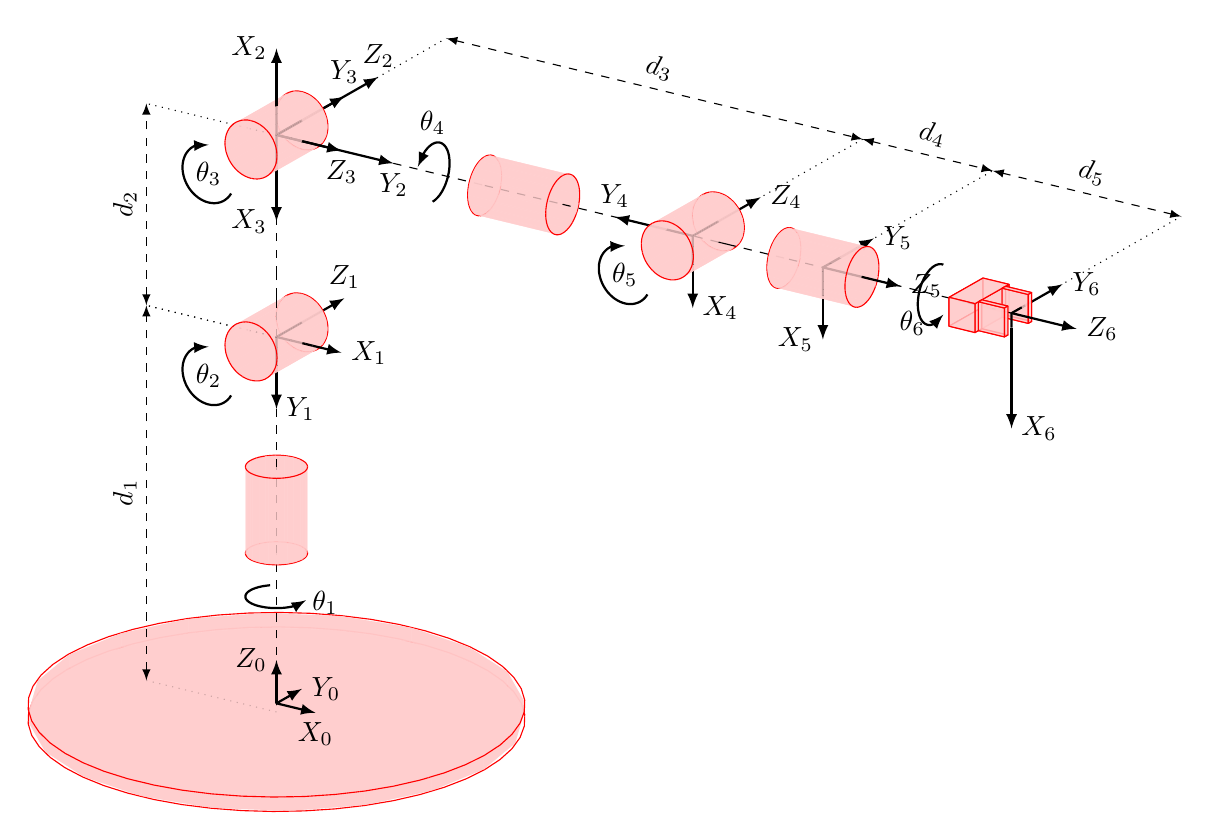
\begin{tikzpicture}[line join=round,scale=0.85]
    [\tikzset{>=latex}]\draw[draw=red](.887,1.23)--(.512,1.258)--(.047,1.271)--(-.115,1.268);
    \draw[draw=red](-.115,1.268)--(-.256,1.266);
    \draw[draw=red](-.256,1.266)--(-.418,1.263)--(-.878,1.232)--(-1.243,1.19);
    \draw[draw=red](1.049,1.214)--(.969,1.224)--(.887,1.23);
    \filldraw[draw=red,fill=red!20,fill opacity=0.8,draw=none](-.185,1.263)--(-.185,1.478)--(.965,1.432)--(.965,1.218)--cycle;
    \draw[draw=red](-1.243,1.19)--(-1.323,1.181)--(-1.4,1.168);
    \filldraw[draw=red,fill=red!20,fill opacity=0.8,draw=none](-1.316,1.175)--(-1.316,1.39)--(-.185,1.478)--(-.185,1.263)--cycle;
    \filldraw[draw=red,fill=red!20,fill opacity=0.8,draw=none](3.095,-.857)--(2.319,-1.176)--(1.316,-1.39)--(.185,-1.478)--(-.965,-1.432)--(-2.02,-1.257)--(-2.877,-.968)--(-3.453,-.596)--(-3.691,-.176)--(-3.567,.251)--(-3.095,.643)--(-2.319,.961)--(-1.316,1.175)--(-.185,1.263)--(.965,1.218)--(2.02,1.042)--(2.877,.754)--(3.453,.382)--(3.691,-.039)--(3.567,-.465)--cycle;
    \draw[draw=red](3.438,.623)--(3.38,.679)--(3.161,.832)--(2.892,.973)--(2.577,1.101)--(2.221,1.213)--(1.831,1.308)--(1.411,1.384)--(.969,1.439)--(.512,1.474)--(.047,1.487)--(-.418,1.478)--(-.878,1.448)--(-1.323,1.397)--(-1.748,1.325)--(-2.145,1.234)--(-2.508,1.125)--(-2.831,1)--(-3.11,.862)--(-3.34,.711)--(-3.517,.551)--(-3.56,.493);
    \draw[draw=red](1.966,1.059)--(1.831,1.092)--(1.411,1.168)--(1.049,1.214);
    \draw[draw=red](2.085,1.031)--(1.966,1.059);
    \filldraw[draw=red,fill=red!20,fill opacity=0.8,draw=none](.965,1.218)--(.965,1.432)--(2.02,1.257)--(2.02,1.042)--cycle;
    \draw[draw=red](-1.4,1.168)--(-1.748,1.109)--(-2.145,1.018)--(-2.271,.981);
    \draw[draw=red](-2.271,.981)--(-2.381,.947);
    \filldraw[draw=red,fill=red!20,fill opacity=0.8,draw=none](-2.319,.961)--(-2.319,1.176)--(-1.316,1.39)--(-1.316,1.175)--cycle;
    \draw[draw=red](2.835,.781)--(2.577,.886)--(2.221,.998)--(2.085,1.031);
    \draw[draw=red](2.94,.732)--(2.892,.758)--(2.835,.781);
    \filldraw[draw=red,fill=red!20,fill opacity=0.8,draw=none](2.02,1.042)--(2.02,1.257)--(2.877,.968)--(2.877,.754)--cycle;
    \draw[draw=red](-2.381,.947)--(-2.508,.91)--(-2.831,.785)--(-3.06,.671);
    \draw[draw=red](-3.06,.671)--(-3.11,.646)--(-3.152,.619);
    \filldraw[draw=red,fill=red!20,fill opacity=0.8,draw=none](-3.095,.643)--(-3.095,.857)--(-2.319,1.176)--(-2.319,.961)--cycle;
    \draw[draw=red](3.438,.407)--(3.38,.464)--(3.161,.616)--(2.94,.732);
    \draw[draw=red](3.489,.358)--(3.438,.407);
    \filldraw[draw=red,fill=red!20,fill opacity=0.8,draw=none](2.877,.754)--(2.877,.968)--(3.453,.596)--(3.453,.382)--cycle;
    \draw[draw=red](-3.152,.619)--(-3.34,.495)--(-3.517,.335)--(-3.56,.277);
    \draw[draw=red](-3.56,.277)--(-3.597,.226);
    \filldraw[draw=red,fill=red!20,fill opacity=0.8,draw=none](-3.567,.251)--(-3.567,.465)--(-3.095,.857)--(-3.095,.643)--cycle;
    \draw[draw=red](3.7,-.008)--(3.657,.133)--(3.546,.302)--(3.489,.358);
    \filldraw[draw=red,fill=red!20,fill opacity=0.8,draw=none](3.453,.382)--(3.453,.596)--(3.691,.176)--(3.691,-.039)--cycle;
    \draw[dotted](0,0)--(-1.944,.471);
    \draw[draw=red](-3.597,.226)--(-3.639,.168)--(-3.703,-.004)--(-3.708,-.146);
    \filldraw[draw=red,fill=red!20,fill opacity=0.8,draw=none](-3.691,-.176)--(-3.691,.039)--(-3.567,.465)--(-3.567,.251)--cycle;
    \draw[dashed](0,.086)--(0,.107);
    \filldraw[draw=red,fill=red!20,fill opacity=0.8,draw=none](3.567,-.251)--(3.691,.176)--(3.453,.596)--(2.877,.968)--(2.02,1.257)--(.965,1.432)--(-.185,1.478)--(-1.316,1.39)--(-2.319,1.176)--(-3.095,.857)--(-3.567,.465)--(-3.691,.039)--(-3.453,-.382)--(-2.877,-.754)--(-2.02,-1.042)--(-.965,-1.218)--(.185,-1.263)--(1.316,-1.175)--(2.319,-.961)--(3.095,-.643)--cycle;
    \draw[draw=red](3.708,.146)--(3.709,.177)--(3.657,.349)--(3.546,.517)--(3.438,.623);
    \draw[draw=red](-3.56,.493)--(-3.639,.383)--(-3.703,.212)--(-3.709,.039)--(-3.7,.008);
    \draw[arrows=<->,thick](.583,-.012)--(0,.129)--(.381,.346);
    \draw[draw=red](3.708,-.07)--(3.709,-.039)--(3.7,-.008);
    \filldraw[draw=red,fill=red!20,fill opacity=0.8,draw=none](3.691,-.039)--(3.691,.176)--(3.567,-.251)--(3.567,-.465)--cycle;
    \draw[draw=red](.062,8.668)--(.081,8.635)--(.114,8.588)--(.152,8.544)--(.16,8.537);
    \filldraw[draw=red,fill=red!20,fill opacity=0.8,draw=none](.151,8.544)--(-.606,8.113)--(-.692,8.229)--(.066,8.66)--cycle;
    \draw[dotted](.379,8.836)--(2.537,10.065);
    \draw[draw=red](3.11,-.862)--(3.34,-.711)--(3.517,-.551)--(3.639,-.383)--(3.703,-.212)--(3.708,-.07);
    \draw[draw=red](3.597,-.226)--(3.639,-.168)--(3.703,.004)--(3.708,.146);
    \draw[dashed](0,.107)--(0,2.374);
    \draw[draw=red](-3.708,-.146)--(-3.709,-.177)--(-3.7,-.208);
    \draw[arrows=->,thick](0,.129)--(0,.776);
    \filldraw[draw=red,fill=red!20,fill opacity=0.8,draw=none](-3.453,-.596)--(-3.453,-.382)--(-3.691,.039)--(-3.691,-.176)--cycle;
    \draw[draw=red](-3.7,-.208)--(-3.657,-.349)--(-3.546,-.517)--(-3.38,-.679)--(-3.161,-.832)--(-2.892,-.973)--(-2.577,-1.101)--(-2.221,-1.213)--(-1.831,-1.308)--(-1.411,-1.384)--(-.969,-1.439)--(-.512,-1.474)--(-.047,-1.487)--(.418,-1.478)--(.878,-1.448)--(1.323,-1.397)--(1.748,-1.325)--(2.145,-1.234)--(2.508,-1.125)--(2.831,-1)--(3.11,-.862);
    \draw[thick](-.095,1.893)--(-.103,1.892)--(-.111,1.892)--(-.119,1.891)--(-.127,1.89)--(-.135,1.889)--(-.142,1.888)--(-.15,1.887)--(-.158,1.886)--(-.165,1.885)--(-.173,1.884)--(-.18,1.883)--(-.188,1.882)--(-.195,1.881)--(-.203,1.879)--(-.21,1.878)--(-.217,1.877)--(-.224,1.875)--(-.231,1.874)--(-.238,1.872)--(-.245,1.871)--(-.252,1.869)--(-.259,1.867)--(-.265,1.866)--(-.272,1.864)--(-.279,1.862)--(-.285,1.86)--(-.291,1.858)--(-.298,1.856)--(-.304,1.855)--(-.31,1.853)--(-.316,1.851)--(-.322,1.848)--(-.328,1.846)--(-.333,1.844)--(-.339,1.842)--(-.344,1.84)--(-.35,1.838)--(-.355,1.835)--(-.36,1.833)--(-.365,1.831)--(-.37,1.828)--(-.375,1.826)--(-.38,1.823)--(-.384,1.821)--(-.389,1.818)--(-.393,1.816)--(-.397,1.813)--(-.402,1.811)--(-.406,1.808)--(-.409,1.805)--(-.413,1.803)--(-.417,1.8)--(-.42,1.797)--(-.424,1.795)--(-.427,1.792)--(-.43,1.789)--(-.433,1.786)--(-.436,1.783)--(-.439,1.781)--(-.441,1.778)--(-.444,1.775)--(-.446,1.772)--(-.448,1.769)--(-.45,1.766)--(-.452,1.763)--(-.454,1.76)--(-.456,1.757)--(-.457,1.754)--(-.458,1.751)--(-.46,1.749)--(-.461,1.746)--(-.462,1.743)--(-.462,1.74)--(-.463,1.737)--(-.464,1.734)--(-.464,1.731)--(-.464,1.728)--(-.464,1.725)--(-.464,1.722)--(-.464,1.719)--(-.464,1.716)--(-.463,1.713)--(-.463,1.71)--(-.462,1.707)--(-.461,1.704)--(-.46,1.701)--(-.459,1.698)--(-.457,1.695)--(-.456,1.692)--(-.454,1.689)--(-.453,1.686)--(-.451,1.683)--(-.449,1.68)--(-.447,1.677)--(-.444,1.674)--(-.442,1.671)--(-.439,1.668)--(-.437,1.666)--(-.434,1.663)--(-.431,1.66)--(-.428,1.657)--(-.425,1.654)--(-.421,1.652)--(-.418,1.649)--(-.414,1.646)--(-.41,1.644)--(-.407,1.641)--(-.403,1.638)--(-.398,1.636)--(-.394,1.633)--(-.39,1.631)--(-.385,1.628)--(-.381,1.626)--(-.376,1.623)--(-.371,1.621)--(-.366,1.618)--(-.361,1.616)--(-.356,1.614)--(-.351,1.611)--(-.346,1.609)--(-.34,1.607)--(-.335,1.605)--(-.329,1.603)--(-.323,1.6)--(-.317,1.598)--(-.311,1.596)--(-.305,1.594)--(-.299,1.592)--(-.293,1.59)--(-.287,1.589)--(-.28,1.587)--(-.274,1.585)--(-.267,1.583)--(-.26,1.581)--(-.254,1.58)--(-.247,1.578)--(-.24,1.577)--(-.233,1.575)--(-.226,1.574)--(-.219,1.572)--(-.212,1.571)--(-.204,1.569)--(-.197,1.568)--(-.19,1.567)--(-.182,1.566)--(-.175,1.564)--(-.167,1.563)--(-.16,1.562)--(-.152,1.561)--(-.144,1.56)--(-.137,1.559)--(-.129,1.559)--(-.121,1.558)--(-.113,1.557)--(-.105,1.556)--(-.098,1.556)--(-.09,1.555)--(-.082,1.554)--(-.074,1.554)--(-.066,1.553)--(-.058,1.553)--(-.05,1.553)--(-.042,1.552)--(-.033,1.552)--(-.025,1.552)--(-.017,1.552)--(-.009,1.552)--(-.001,1.552)--(.007,1.552)--(.015,1.552)--(.023,1.552)--(.031,1.552)--(.039,1.552)--(.047,1.553)--(.056,1.553)--(.064,1.553)--(.072,1.554)--(.08,1.554)--(.088,1.555)--(.095,1.555)--(.103,1.556)--(.111,1.557)--(.119,1.557)--(.127,1.558)--(.135,1.559)--(.142,1.56)--(.15,1.561)--(.158,1.562)--(.165,1.563)--(.173,1.564)--(.18,1.565)--(.188,1.566)--(.195,1.568)--(.203,1.569)--(.21,1.57)--(.217,1.572)--(.224,1.573)--(.231,1.575)--(.238,1.576)--(.245,1.578)--(.252,1.579)--(.259,1.581)--(.265,1.583)--(.272,1.584)--(.279,1.586)--(.285,1.588)--(.291,1.59)--(.298,1.592)--(.304,1.594)--(.31,1.596)--(.316,1.598)--(.322,1.6)--(.328,1.602)--(.333,1.604)--(.339,1.606);
    \draw[draw=red](-3.7,.008)--(-3.657,-.133)--(-3.546,-.302)--(-3.489,-.358);
    \draw[draw=red](.354,2.482)--(.322,2.495)--(.278,2.509)--(.229,2.521)--(.176,2.53)--(.121,2.537)--(.064,2.541)--(.006,2.543)--(-.052,2.542)--(-.11,2.538)--(-.165,2.532)--(-.218,2.523)--(-.268,2.511)--(-.313,2.498)--(-.354,2.482)--(-.382,2.468);
    \draw[draw=red](.436,2.429)--(.423,2.442)--(.395,2.461)--(.361,2.479)--(.354,2.482);
    \draw[draw=red](-.382,2.468)--(-.389,2.465)--(-.418,2.446)--(-.44,2.426)--(-.445,2.419);
    \filldraw[draw=red,fill=red!20,fill opacity=0.8,draw=none](.387,2.28)--(.29,2.24)--(.165,2.214)--(.023,2.203)--(-.121,2.208)--(-.252,2.23)--(-.36,2.266)--(-.432,2.313)--(-.461,2.365)--(-.446,2.419)--(-.387,2.468)--(-.29,2.507)--(-.165,2.534)--(-.023,2.545)--(.121,2.54)--(.252,2.518)--(.36,2.482)--(.432,2.435)--(.461,2.383)--(.446,2.329)--cycle;
    \filldraw[draw=red,fill=red!20,fill opacity=0.8,draw=none](-.165,2.534)--(-.165,3.821)--(-.023,3.832)--(-.023,2.545)--cycle;
    \filldraw[draw=red,fill=red!20,fill opacity=0.8,draw=none](-.023,2.545)--(-.023,3.832)--(.121,3.826)--(.121,2.54)--cycle;
    \filldraw[draw=red,fill=red!20,fill opacity=0.8,draw=none](.121,2.54)--(.121,3.826)--(.252,3.804)--(.252,2.518)--cycle;
    \filldraw[draw=red,fill=red!20,fill opacity=0.8,draw=none](-.29,2.507)--(-.29,3.794)--(-.165,3.821)--(-.165,2.534)--cycle;
    \filldraw[draw=red,fill=red!20,fill opacity=0.8,draw=none](.252,2.518)--(.252,3.804)--(.36,3.768)--(.36,2.482)--cycle;
    \filldraw[draw=red,fill=red!20,fill opacity=0.8,draw=none](-.387,2.468)--(-.387,3.754)--(-.29,3.794)--(-.29,2.507)--cycle;
    \filldraw[draw=red,fill=red!20,fill opacity=0.8,draw=none](.36,2.482)--(.36,3.768)--(.432,3.722)--(.432,2.435)--cycle;
    \filldraw[draw=red,fill=red!20,fill opacity=0.8,draw=none](-.446,2.419)--(-.446,3.705)--(-.387,3.754)--(-.387,2.468)--cycle;
    \draw[draw=red](.462,2.383)--(.457,2.401)--(.443,2.422)--(.436,2.429);
    \filldraw[draw=red,fill=red!20,fill opacity=0.8,draw=none](.432,2.435)--(.432,3.722)--(.461,3.669)--(.461,2.383)--cycle;
    \draw[draw=red](.159,5.521)--(.133,5.548)--(.097,5.594)--(.066,5.643)--(.061,5.652);
    \filldraw[draw=red,fill=red!20,fill opacity=0.8,draw=none](-.692,5.212)--(.066,5.643)--(.151,5.527)--(-.606,5.096)--cycle;
    \draw[arrows=->,thick](.379,5.819)--(1.015,6.181);
    \draw[thick,->](.31,1.596)--(.441,1.67);
    \draw[draw=red](-.445,2.419)--(-.45,2.412);
    \draw[draw=red](-.45,2.412)--(-.455,2.405)--(-.463,2.384)--(-.464,2.366);
    \filldraw[draw=red,fill=red!20,fill opacity=0.8,draw=none](-.461,2.365)--(-.461,3.652)--(-.446,3.705)--(-.446,2.419)--cycle;
    \filldraw[draw=red,fill=red!20,fill opacity=0.8,draw=none](3.567,-.465)--(3.567,-.251)--(3.095,-.643)--(3.095,-.857)--cycle;
    \draw[draw=red](3.56,-.277)--(3.597,-.226);
    \draw[draw=red](.464,2.375)--(.464,2.379)--(.462,2.383);
    \filldraw[draw=red,fill=red!20,fill opacity=0.8,draw=none](.461,2.383)--(.461,3.669)--(.446,3.616)--(.446,2.329)--cycle;
    \draw[draw=red](.389,2.276)--(.418,2.295)--(.44,2.315)--(.455,2.336)--(.463,2.358)--(.464,2.375);
    \draw[dashed](0,2.374)--(0,3.661);
    \draw[draw=red](-.464,2.366)--(-.464,2.362)--(-.462,2.358);
    \filldraw[draw=red,fill=red!20,fill opacity=0.8,draw=none](-.432,2.313)--(-.432,3.599)--(-.461,3.652)--(-.461,2.365)--cycle;
    \draw[draw=red](-.462,2.358)--(-.457,2.341)--(-.443,2.32)--(-.423,2.299)--(-.395,2.28)--(-.361,2.262)--(-.322,2.247)--(-.278,2.233)--(-.229,2.221)--(-.176,2.211)--(-.121,2.204)--(-.064,2.2)--(-.006,2.198)--(.052,2.199)--(.11,2.203)--(.165,2.21)--(.218,2.219)--(.268,2.23)--(.313,2.244)--(.354,2.259)--(.389,2.276);
    \draw[draw=red](3.11,-.646)--(3.34,-.495)--(3.517,-.335)--(3.56,-.277);
    \draw[draw=red](.354,3.775)--(.322,3.788)--(.278,3.802)--(.229,3.814)--(.176,3.823)--(.121,3.83)--(.064,3.835)--(.006,3.836)--(-.014,3.836);
    \draw[draw=red](-.014,3.836)--(-.052,3.835)--(-.11,3.831)--(-.165,3.825)--(-.175,3.823);
    \filldraw[draw=red,fill=red!20,fill opacity=0.8,draw=none](.446,3.616)--(.461,3.669)--(.432,3.722)--(.36,3.768)--(.252,3.804)--(.121,3.826)--(-.023,3.832)--(-.165,3.821)--(-.29,3.794)--(-.387,3.754)--(-.446,3.705)--(-.461,3.652)--(-.432,3.599)--(-.36,3.553)--(-.252,3.517)--(-.121,3.495)--(.023,3.489)--(.165,3.5)--(.29,3.527)--(.387,3.567)--cycle;
    \filldraw[draw=red,fill=red!20,fill opacity=0.8,draw=none](.446,2.329)--(.446,3.616)--(.387,3.567)--(.387,2.28)--cycle;
    \draw[dotted](-.54,5.734)--(-1.944,6.075);
    \draw[dotted](-.54,5.734)--(-1.944,6.075);
    \draw[draw=red](-.175,3.823)--(-.218,3.816)--(-.268,3.805)--(-.298,3.796);
    \filldraw[draw=red,fill=red!20,fill opacity=0.8,draw=none](-.36,2.266)--(-.36,3.553)--(-.432,3.599)--(-.432,2.313)--cycle;
    \draw[draw=red](-.298,3.796)--(-.313,3.791)--(-.354,3.775)--(-.389,3.758)--(-.394,3.755);
    \filldraw[draw=red,fill=red!20,fill opacity=0.8,draw=none](-2.877,-.968)--(-2.877,-.754)--(-3.453,-.382)--(-3.453,-.596)--cycle;
    \filldraw[draw=red,fill=red!20,fill opacity=0.8,draw=none](.387,2.28)--(.387,3.567)--(.29,3.527)--(.29,2.24)--cycle;
    \draw[draw=red](.436,3.722)--(.423,3.735)--(.395,3.754)--(.361,3.772)--(.354,3.775);
    \draw[draw=red](-3.489,-.358)--(-3.438,-.407);
    \filldraw[draw=red,fill=red!20,fill opacity=0.8,draw=none](-.252,2.23)--(-.252,3.517)--(-.36,3.553)--(-.36,2.266)--cycle;
    \draw[draw=red](-.394,3.755)--(-.418,3.739)--(-.44,3.719)--(-.45,3.706);
    \draw[arrows=->,thick](.379,8.836)--(1.522,9.487);
    \filldraw[draw=red,fill=red!20,fill opacity=0.8,draw=none](.29,2.24)--(.29,3.527)--(.165,3.5)--(.165,2.214)--cycle;
    \filldraw[draw=red,fill=red!20,fill opacity=0.8,draw=none](-.121,2.208)--(-.121,3.495)--(-.252,3.517)--(-.252,2.23)--cycle;
    \draw[draw=red](.464,3.669)--(.464,3.672)--(.457,3.694)--(.443,3.715)--(.436,3.722);
    \draw[draw=red](-3.438,-.407)--(-3.38,-.464)--(-3.161,-.616)--(-2.94,-.732);
    \filldraw[draw=red,fill=red!20,fill opacity=0.8,draw=none](.165,2.214)--(.165,3.5)--(.023,3.489)--(.023,2.203)--cycle;
    \draw[draw=red](-.45,3.706)--(-.455,3.698)--(-.463,3.677)--(-.464,3.655)--(-.462,3.651);
    \filldraw[draw=red,fill=red!20,fill opacity=0.8,draw=none](.023,2.203)--(.023,3.489)--(-.121,3.495)--(-.121,2.208)--cycle;
    \draw[draw=red](.061,5.652)--(.04,5.695)--(.019,5.749)--(.009,5.785);
    \filldraw[draw=red,fill=red!20,fill opacity=0.8,draw=none](-.747,5.345)--(.011,5.776)--(.066,5.643)--(-.692,5.212)--cycle;
    \filldraw[draw=red,fill=red!20,fill opacity=0.8,draw=none](.747,5.597)--(.692,5.491)--(.606,5.417)--(.498,5.382)--(.379,5.39)--(.259,5.44)--(.151,5.527)--(.066,5.643)--(.011,5.776)--(-.008,5.913)--(.011,6.041)--(.066,6.147)--(.151,6.221)--(.259,6.256)--(.379,6.248)--(.498,6.198)--(.606,6.111)--(.692,5.995)--(.747,5.862)--(.766,5.725)--cycle;
    \draw[draw=red](.252,5.445)--(.215,5.47)--(.172,5.507)--(.159,5.521);
    \draw[draw=red](.009,5.785)--(.004,5.804)--(-.005,5.859)--(-.008,5.904);
    \filldraw[draw=red,fill=red!20,fill opacity=0.8,draw=none](-.606,5.096)--(.151,5.527)--(.259,5.44)--(-.498,5.009)--cycle;
    \filldraw[draw=red,fill=red!20,fill opacity=0.8,draw=none](-.766,5.482)--(-.008,5.913)--(.011,5.776)--(-.747,5.345)--cycle;
    \draw[draw=red](.445,3.616)--(.455,3.629)--(.463,3.651)--(.464,3.669);
    \draw[draw=red](.269,5.435)--(.26,5.439)--(.252,5.445);
    \draw[draw=red](-.008,5.904)--(-.008,5.914)--(-.008,5.924);
    \draw[dashed](0,3.661)--(0,5.004);
    \draw[draw=red](.373,5.392)--(.356,5.396)--(.308,5.414)--(.269,5.435);
    \filldraw[draw=red,fill=red!20,fill opacity=0.8,draw=none](-.498,5.009)--(.259,5.44)--(.379,5.39)--(-.379,4.959)--cycle;
    \draw[draw=red](-.008,5.924)--(-.005,5.968)--(.004,6.018)--(.009,6.035);
    \draw[dotted](-.429,5.707)--(-.54,5.734);
    \draw[dotted](-.429,5.707)--(-.54,5.734);
    \draw[dotted](-.387,5.697)--(-.429,5.707);
    \draw[dotted](-.387,5.697)--(-.429,5.707);
    \filldraw[draw=red,fill=red!20,fill opacity=0.8,draw=none](-.747,5.61)--(.011,6.041)--(-.008,5.913)--(-.766,5.482)--cycle;
    \draw[draw=red](-.462,3.651)--(-.457,3.634)--(-.443,3.613)--(-.43,3.599);
    \draw[draw=red](.388,5.388)--(.373,5.392);
    \draw[draw=red](.009,6.035)--(.014,6.05);
    \draw[draw=red](.492,5.381)--(.453,5.379)--(.405,5.384)--(.388,5.388);
    \draw[draw=red](.509,5.383)--(.501,5.381)--(.492,5.381);
    \draw[arrows=-,thick](0,5.128)--(0,5.004);
    \draw[dashed](0,5.004)--(0,5.128);
    \draw[arrows=-,thick](0,5.175)--(0,5.128);
    \draw[dashed](0,5.128)--(0,5.172);
    \filldraw[draw=red,fill=red!20,fill opacity=0.8,draw=none](-.379,4.959)--(.379,5.39)--(.498,5.382)--(-.259,4.951)--cycle;
    \draw[draw=red](.014,6.05)--(.019,6.066)--(.04,6.11)--(.061,6.143);
    \draw[draw=red](.061,6.143)--(.066,6.15)--(.072,6.156);
    \filldraw[draw=red,fill=red!20,fill opacity=0.8,draw=none](-.692,5.716)--(.066,6.147)--(.011,6.041)--(-.747,5.61)--cycle;
    \draw[draw=red](.389,3.57)--(.418,3.588)--(.44,3.608)--(.445,3.616);
    \draw[draw=red](.603,5.413)--(.589,5.406)--(.546,5.39)--(.509,5.383);
    \filldraw[draw=red,fill=red!20,fill opacity=0.8,draw=none](-.259,4.951)--(.498,5.382)--(.606,5.417)--(-.151,4.986)--cycle;
    \draw[draw=red](.072,6.156)--(.097,6.184)--(.133,6.212)--(.147,6.22);
    \filldraw[draw=red,fill=red!20,fill opacity=0.8,draw=none](-.606,5.79)--(.151,6.221)--(.066,6.147)--(-.692,5.716)--cycle;
    \draw[draw=red](-.43,3.599)--(-.423,3.592)--(-.395,3.573)--(-.361,3.556)--(-.354,3.553);
    \draw[draw=red](.615,5.42)--(.603,5.413);
    \draw[draw=red](.147,6.22)--(.159,6.227);
    \draw[draw=red](-.354,3.553)--(-.322,3.54)--(-.278,3.526)--(-.229,3.514)--(-.176,3.504)--(-.121,3.497)--(-.064,3.493)--(-.006,3.491)--(.052,3.492)--(.11,3.496)--(.165,3.503)--(.218,3.512)--(.268,3.523)--(.313,3.537)--(.354,3.552)--(.389,3.57);
    \filldraw[draw=red,fill=red!20,fill opacity=0.8,draw=none](-.151,4.986)--(.606,5.417)--(.692,5.491)--(-.066,5.06)--cycle;
    \draw[arrows=-,thick](0,5.603)--(.379,5.819);
    \filldraw[draw=red,fill=red!20,fill opacity=0.8,draw=none](-.498,5.825)--(.259,6.256)--(.151,6.221)--(-.606,5.79)--cycle;
    \draw[draw=red](.769,5.726)--(.766,5.673)--(.757,5.622)--(.742,5.574)--(.721,5.53)--(.695,5.49)--(.664,5.456)--(.628,5.428)--(.615,5.42);
    \draw[draw=red](.159,6.227)--(.172,6.234)--(.215,6.25)--(.26,6.259)--(.308,6.261)--(.356,6.256)--(.405,6.244)--(.453,6.226)--(.501,6.201)--(.546,6.17)--(.589,6.133)--(.628,6.092)--(.664,6.046)--(.695,5.997)--(.721,5.945)--(.742,5.891)--(.757,5.836)--(.766,5.781)--(.769,5.726);
    \filldraw[draw=red,fill=red!20,fill opacity=0.8,draw=none](-.066,5.06)--(.692,5.491)--(.747,5.597)--(-.011,5.166)--cycle;
    \filldraw[draw=red,fill=red!20,fill opacity=0.8,draw=none](-.379,5.817)--(.379,6.248)--(.259,6.256)--(-.498,5.825)--cycle;
    \draw[arrows=->,thick](0,5.004)--(0,4.526);
    \filldraw[draw=red,fill=red!20,fill opacity=0.8,draw=none](3.095,-.857)--(3.095,-.643)--(2.319,-.961)--(2.319,-1.176)--cycle;
    \draw[arrows=-,thick](.387,5.51)--(0,5.603)--(0,5.175);
    \filldraw[draw=red,fill=red!20,fill opacity=0.8,draw=none](-.011,5.166)--(.747,5.597)--(.766,5.725)--(.008,5.294)--cycle;
    \draw[dashed](0,5.603)--(0,6.032);
    \filldraw[draw=red,fill=red!20,fill opacity=0.8,draw=none](-.259,5.767)--(.498,6.198)--(.379,6.248)--(-.379,5.817)--cycle;
    \draw[draw=red](3.06,-.671)--(3.11,-.646);
    \filldraw[draw=red,fill=red!20,fill opacity=0.8,draw=none](.008,5.294)--(.766,5.725)--(.747,5.862)--(-.011,5.431)--cycle;
    \filldraw[draw=red,fill=red!20,fill opacity=0.8,draw=none](-.151,5.68)--(.606,6.111)--(.498,6.198)--(-.259,5.767)--cycle;
    \filldraw[draw=red,fill=red!20,fill opacity=0.8,draw=none](-.011,5.431)--(.747,5.862)--(.692,5.995)--(-.066,5.564)--cycle;
    \draw[dotted](0,5.603)--(-.387,5.697);
    \draw[dotted](0,5.603)--(-.387,5.697);
    \filldraw[draw=red,fill=red!20,fill opacity=0.8,draw=none](-.066,5.564)--(.692,5.995)--(.606,6.111)--(-.151,5.68)--cycle;
    \draw[draw=red](2.381,-.947)--(2.508,-.91)--(2.831,-.785)--(3.06,-.671);
    \draw[arrows=->,thick](.379,8.836)--(1.015,9.198);
    \filldraw[draw=red,fill=red!20,fill opacity=0.8,draw=none](-2.02,-1.257)--(-2.02,-1.042)--(-2.877,-.754)--(-2.877,-.968)--cycle;
    \draw[draw=red](-2.94,-.732)--(-2.892,-.758)--(-2.835,-.781);
    \draw[draw=red](-2.835,-.781)--(-2.577,-.886)--(-2.221,-.998)--(-2.085,-1.031);
    \draw[dotted](-.54,8.752)--(-1.944,9.092);
    \draw[dashed](0,6.032)--(0,6.079);
    \draw[dashed](0,6.079)--(0,6.203);
    \draw[arrows=-,thick](.429,5.5)--(.387,5.51);
    \draw[dashed](0,6.203)--(0,6.537);
    \filldraw[draw=red,fill=red!20,fill opacity=0.8,draw=none](.008,5.294)--(-.011,5.431)--(-.066,5.564)--(-.151,5.68)--(-.259,5.767)--(-.379,5.817)--(-.498,5.825)--(-.606,5.79)--(-.692,5.716)--(-.747,5.61)--(-.766,5.482)--(-.747,5.345)--(-.692,5.212)--(-.606,5.096)--(-.498,5.009)--(-.379,4.959)--(-.259,4.951)--(-.151,4.986)--(-.066,5.06)--(-.011,5.166)--cycle;
    \draw[draw=red](-.603,5.088)--(-.628,5.115)--(-.664,5.16)--(-.695,5.21)--(-.7,5.219);
    \draw[draw=red](-.7,5.219)--(-.721,5.262)--(-.742,5.316)--(-.752,5.352);
    \draw[arrows=-,thick](.54,5.472)--(.429,5.5);
    \draw[draw=red](-.509,5.012)--(-.546,5.037)--(-.589,5.073)--(-.603,5.088);
    \draw[draw=red](-.752,5.352)--(-.757,5.371)--(-.766,5.426)--(-.769,5.481)--(-.769,5.491);
    \draw[draw=red](-.373,4.955)--(-.405,4.963)--(-.453,4.981)--(-.501,5.006)--(-.509,5.012);
    \draw[draw=red](-.769,5.491)--(-.766,5.534)--(-.757,5.585)--(-.747,5.617);
    \draw[arrows=<-,thick](.972,5.368)--(.54,5.472);
    \draw[dashed](0,6.537)--(0,8.022);
    \draw[draw=red](-.252,4.949)--(-.26,4.948)--(-.308,4.946)--(-.356,4.951)--(-.373,4.955);
    \draw[draw=red](.009,8.804)--(.011,8.794)--(.029,8.739)--(.052,8.686)--(.062,8.668);
    \draw[draw=red](-.747,5.617)--(-.742,5.633)--(-.721,5.677)--(-.695,5.716)--(-.689,5.723);
    \filldraw[draw=red,fill=red!20,fill opacity=0.8,draw=none](.066,8.66)--(-.692,8.229)--(-.747,8.362)--(.011,8.793)--cycle;
    \filldraw[draw=red,fill=red!20,fill opacity=0.8,draw=none](.379,8.407)--(.259,8.457)--(.151,8.544)--(.066,8.66)--(.011,8.793)--(-.008,8.93)--(.011,9.058)--(.066,9.164)--(.151,9.238)--(.259,9.273)--(.379,9.265)--(.498,9.215)--(.606,9.128)--(.692,9.012)--(.747,8.88)--(.766,8.742)--(.747,8.614)--(.692,8.508)--(.606,8.434)--(.498,8.399)--cycle;
    \filldraw[draw=red,fill=red!20,fill opacity=0.8,draw=none](2.319,-1.176)--(2.319,-.961)--(1.316,-1.175)--(1.316,-1.39)--cycle;
    \draw[draw=red](.16,8.537)--(.193,8.505)--(.237,8.471)--(.268,8.453);
    \draw[draw=red](-.007,8.94)--(-.007,8.904)--(-.001,8.849)--(.009,8.804);
    \filldraw[draw=red,fill=red!20,fill opacity=0.8,draw=none](.259,8.457)--(-.498,8.026)--(-.606,8.113)--(.151,8.544)--cycle;
    \filldraw[draw=red,fill=red!20,fill opacity=0.8,draw=none](.011,8.793)--(-.747,8.362)--(-.766,8.499)--(-.008,8.93)--cycle;
    \draw[draw=red](.268,8.453)--(.284,8.443)--(.332,8.421)--(.381,8.406);
    \filldraw[draw=red,fill=red!20,fill opacity=0.8,draw=none](.379,8.407)--(-.379,7.976)--(-.498,8.026)--(.259,8.457)--cycle;
    \draw[draw=red](.009,9.051)--(-.001,9.011)--(-.007,8.958)--(-.007,8.94);
    \draw[draw=red](.014,9.068)--(.011,9.06)--(.009,9.051);
    \draw[dotted](-.429,8.725)--(-.54,8.752);
    \draw[dotted](-.387,8.714)--(-.429,8.725);
    \filldraw[draw=red,fill=red!20,fill opacity=0.8,draw=none](-.008,8.93)--(-.766,8.499)--(-.747,8.627)--(.011,9.058)--cycle;
    \draw[draw=red](2.271,-.981)--(2.381,-.947);
    \draw[draw=red](-.147,4.987)--(-.172,4.972)--(-.215,4.957)--(-.252,4.949);
    \draw[draw=red](-.689,5.723)--(-.664,5.751)--(-.628,5.779)--(-.603,5.794);
    \draw[draw=red](.381,8.406)--(.429,8.398)--(.477,8.396)--(.493,8.398);
    \draw[draw=red](.493,8.398)--(.508,8.4);
    \draw[dashed](0,8.022)--(0,8.145);
    \draw[arrows=-,thick](0,8.022)--(0,8.145);
    \draw[dashed](0,8.145)--(0,8.192);
    \draw[arrows=-,thick](0,8.145)--(0,8.192);
    \filldraw[draw=red,fill=red!20,fill opacity=0.8,draw=none](.498,8.399)--(-.259,7.968)--(-.379,7.976)--(.379,8.407)--cycle;
    \draw[draw=red](.062,9.161)--(.052,9.148)--(.029,9.106)--(.014,9.068);
    \draw[draw=red](.071,9.172)--(.062,9.161);
    \filldraw[draw=red,fill=red!20,fill opacity=0.8,draw=none](.011,9.058)--(-.747,8.627)--(-.692,8.733)--(.066,9.164)--cycle;
    \draw[draw=red](1.4,-1.168)--(1.748,-1.109)--(2.145,-1.018)--(2.271,-.981);
    \draw[draw=red](-.072,5.051)--(-.097,5.023)--(-.133,4.995)--(-.147,4.987);
    \draw[draw=red](-.603,5.794)--(-.589,5.801)--(-.546,5.817)--(-.509,5.824);
    \draw[draw=red](.508,8.4)--(.524,8.402)--(.568,8.414)--(.602,8.43);
    \filldraw[draw=red,fill=red!20,fill opacity=0.8,draw=none](.606,8.434)--(-.151,8.003)--(-.259,7.968)--(.498,8.399)--cycle;
    \draw[draw=red](.145,9.237)--(.114,9.216)--(.081,9.185)--(.071,9.172);
    \filldraw[draw=red,fill=red!20,fill opacity=0.8,draw=none](.066,9.164)--(-.692,8.733)--(-.606,8.807)--(.151,9.238)--cycle;
    \filldraw[draw=red,fill=red!20,fill opacity=0.8,draw=none](-.965,-1.432)--(-.965,-1.218)--(-2.02,-1.042)--(-2.02,-1.257)--cycle;
    \draw[draw=red](-.061,5.064)--(-.066,5.057)--(-.072,5.051);
    \draw[draw=red](-.509,5.824)--(-.501,5.826)--(-.492,5.826);
    \draw[draw=red](-.009,5.172)--(-.019,5.141)--(-.04,5.097)--(-.061,5.064);
    \draw[draw=red](-.492,5.826)--(-.453,5.828)--(-.405,5.823)--(-.373,5.815);
    \draw[draw=red](-2.085,-1.031)--(-1.966,-1.059);
    \draw[draw=red](.602,8.43)--(.609,8.433)--(.616,8.438);
    \draw[draw=red](.16,9.245)--(.152,9.241)--(.145,9.237);
    \filldraw[draw=red,fill=red!20,fill opacity=0.8,draw=none](.692,8.508)--(-.066,8.077)--(-.151,8.003)--(.606,8.434)--cycle;
    \draw[arrows=-,thick](0,8.192)--(0,8.621)--(.379,8.836);
    \draw[arrows=-,thick](0,8.621)--(.379,8.836);
    \draw[dotted](0,8.621)--(.379,8.836);
    \filldraw[draw=red,fill=red!20,fill opacity=0.8,draw=none](.151,9.238)--(-.606,8.807)--(-.498,8.842)--(.259,9.273)--cycle;
    \draw[draw=red](.616,8.438)--(.647,8.459)--(.68,8.49)--(.709,8.527)--(.732,8.568)--(.75,8.614)--(.762,8.664)--(.769,8.716)--(.769,8.77)--(.762,8.825)--(.75,8.881)--(.732,8.936)--(.709,8.989)--(.68,9.039)--(.647,9.087)--(.609,9.131)--(.568,9.17)--(.524,9.203)--(.477,9.231)--(.429,9.253)--(.381,9.268)--(.332,9.277)--(.284,9.278)--(.237,9.273)--(.193,9.26)--(.16,9.245);
    \draw[arrows=<-,thick](0,7.328)--(0,8.022);
    \draw[draw=red](.008,5.293)--(.005,5.239)--(-.004,5.188)--(-.009,5.172);
    \draw[draw=red](-.373,5.815)--(-.356,5.811)--(-.308,5.793)--(-.26,5.768)--(-.252,5.762);
    \draw[draw=red](-1.966,-1.059)--(-1.831,-1.092)--(-1.411,-1.168)--(-1.049,-1.214);
    \filldraw[draw=red,fill=red!20,fill opacity=0.8,draw=none](.747,8.614)--(-.011,8.183)--(-.066,8.077)--(.692,8.508)--cycle;
    \filldraw[draw=red,fill=red!20,fill opacity=0.8,draw=none](.259,9.273)--(-.498,8.842)--(-.379,8.834)--(.379,9.265)--cycle;
    \draw[draw=red](-.014,5.439)--(-.004,5.403)--(.005,5.347)--(.008,5.293);
    \draw[draw=red](-.252,5.762)--(-.215,5.737)--(-.172,5.7)--(-.147,5.673);
    \draw[draw=red](-.072,5.573)--(-.066,5.564)--(-.04,5.512)--(-.019,5.458)--(-.014,5.439);
    \draw[draw=red](-.147,5.673)--(-.133,5.659)--(-.097,5.613)--(-.072,5.573);
    \draw[dashed](0,8.192)--(0,8.621);
    \filldraw[draw=red,fill=red!20,fill opacity=0.8,draw=none](.766,8.742)--(.008,8.311)--(-.011,8.183)--(.747,8.614)--cycle;
    \draw[arrows=-,thick](0,9.05)--(0,8.621)--(.387,8.527);
    \filldraw[draw=red,fill=red!20,fill opacity=0.8,draw=none](.379,9.265)--(-.379,8.834)--(-.259,8.784)--(.498,9.215)--cycle;
    \draw[dashed](0,8.621)--(.387,8.527);
    \draw[arrows=-,thick](0,8.621)--(.387,8.527);
    \filldraw[draw=red,fill=red!20,fill opacity=0.8,draw=none](.747,8.88)--(-.011,8.449)--(.008,8.311)--(.766,8.742)--cycle;
    \filldraw[draw=red,fill=red!20,fill opacity=0.8,draw=none](.498,9.215)--(-.259,8.784)--(-.151,8.697)--(.606,9.128)--cycle;
    \filldraw[draw=red,fill=red!20,fill opacity=0.8,draw=none](1.316,-1.39)--(1.316,-1.175)--(.185,-1.263)--(.185,-1.478)--cycle;
    \filldraw[draw=red,fill=red!20,fill opacity=0.8,draw=none](.692,9.012)--(-.066,8.581)--(-.011,8.449)--(.747,8.88)--cycle;
    \draw[dotted](0,8.621)--(-.387,8.714);
    \filldraw[draw=red,fill=red!20,fill opacity=0.8,draw=none](.606,9.128)--(-.151,8.697)--(-.066,8.581)--(.692,9.012)--cycle;
    \draw[draw=red](1.243,-1.19)--(1.323,-1.181)--(1.4,-1.168);
    \filldraw[draw=red,fill=red!20,fill opacity=0.8,draw=none](.185,-1.478)--(.185,-1.263)--(-.965,-1.218)--(-.965,-1.432)--cycle;
    \draw[draw=red](.256,-1.266)--(.418,-1.263)--(.878,-1.232)--(1.243,-1.19);
    \draw[draw=red](-1.049,-1.214)--(-.969,-1.224)--(-.887,-1.23);
    \draw[draw=red](-.887,-1.23)--(-.512,-1.258)--(-.047,-1.271)--(.115,-1.268);
    \draw[thick](-.678,4.729)--(-.682,4.723)--(-.685,4.718)--(-.689,4.712)--(-.693,4.707)--(-.696,4.701)--(-.7,4.696)--(-.704,4.691)--(-.709,4.686)--(-.713,4.681)--(-.717,4.677)--(-.721,4.672)--(-.726,4.667)--(-.731,4.663)--(-.735,4.659)--(-.74,4.654)--(-.745,4.65)--(-.75,4.646)--(-.755,4.643)--(-.76,4.639)--(-.765,4.635)--(-.77,4.632)--(-.776,4.628)--(-.781,4.625)--(-.786,4.622)--(-.792,4.619)--(-.798,4.616)--(-.803,4.613)--(-.809,4.61)--(-.815,4.608)--(-.821,4.606)--(-.826,4.603)--(-.832,4.601)--(-.838,4.599)--(-.844,4.597)--(-.851,4.595)--(-.857,4.594)--(-.863,4.592)--(-.869,4.591)--(-.876,4.59)--(-.882,4.589)--(-.888,4.588)--(-.895,4.587)--(-.901,4.586)--(-.908,4.586)--(-.914,4.585)--(-.921,4.585)--(-.927,4.585)--(-.934,4.585)--(-.941,4.585)--(-.947,4.585)--(-.954,4.585)--(-.961,4.586)--(-.968,4.587)--(-.974,4.587)--(-.981,4.588)--(-.988,4.589)--(-.995,4.591)--(-1.001,4.592)--(-1.008,4.593)--(-1.015,4.595)--(-1.022,4.597)--(-1.028,4.598)--(-1.035,4.6)--(-1.042,4.602)--(-1.049,4.605)--(-1.056,4.607)--(-1.062,4.61)--(-1.069,4.612)--(-1.076,4.615)--(-1.082,4.618)--(-1.089,4.621)--(-1.096,4.624)--(-1.102,4.627)--(-1.109,4.63)--(-1.116,4.634)--(-1.122,4.638)--(-1.129,4.641)--(-1.135,4.645)--(-1.141,4.649)--(-1.148,4.653)--(-1.154,4.657)--(-1.161,4.662)--(-1.167,4.666)--(-1.173,4.67)--(-1.179,4.675)--(-1.185,4.68)--(-1.191,4.685)--(-1.197,4.69)--(-1.203,4.695)--(-1.209,4.7)--(-1.215,4.705)--(-1.221,4.71)--(-1.227,4.716)--(-1.232,4.721)--(-1.238,4.727)--(-1.243,4.733)--(-1.249,4.738)--(-1.254,4.744)--(-1.26,4.75)--(-1.265,4.756)--(-1.27,4.762)--(-1.275,4.769)--(-1.28,4.775)--(-1.285,4.781)--(-1.29,4.788)--(-1.295,4.794)--(-1.299,4.801)--(-1.304,4.808)--(-1.308,4.814)--(-1.313,4.821)--(-1.317,4.828)--(-1.321,4.835)--(-1.325,4.842)--(-1.329,4.849)--(-1.333,4.856)--(-1.337,4.863)--(-1.341,4.87)--(-1.345,4.877)--(-1.348,4.885)--(-1.352,4.892)--(-1.355,4.899)--(-1.358,4.907)--(-1.361,4.914)--(-1.364,4.922)--(-1.367,4.929)--(-1.37,4.937)--(-1.373,4.944)--(-1.375,4.952)--(-1.378,4.959)--(-1.38,4.967)--(-1.382,4.975)--(-1.385,4.982)--(-1.387,4.99)--(-1.389,4.998)--(-1.39,5.005)--(-1.392,5.013)--(-1.394,5.021)--(-1.395,5.028)--(-1.397,5.036)--(-1.398,5.044)--(-1.399,5.052)--(-1.4,5.059)--(-1.401,5.067)--(-1.402,5.075)--(-1.402,5.082)--(-1.403,5.09)--(-1.403,5.097)--(-1.403,5.105)--(-1.404,5.113)--(-1.404,5.12)--(-1.404,5.128)--(-1.403,5.135)--(-1.403,5.143)--(-1.403,5.15)--(-1.402,5.157)--(-1.402,5.165)--(-1.401,5.172)--(-1.4,5.179)--(-1.399,5.186)--(-1.398,5.194)--(-1.397,5.201)--(-1.395,5.208)--(-1.394,5.215)--(-1.392,5.222)--(-1.39,5.228)--(-1.389,5.235)--(-1.387,5.242)--(-1.385,5.249)--(-1.382,5.255)--(-1.38,5.262)--(-1.378,5.268)--(-1.375,5.275)--(-1.373,5.281)--(-1.37,5.287)--(-1.367,5.293)--(-1.364,5.3)--(-1.361,5.306)--(-1.358,5.311)--(-1.355,5.317)--(-1.352,5.323)--(-1.348,5.329)--(-1.345,5.334)--(-1.341,5.34)--(-1.337,5.345)--(-1.333,5.35)--(-1.329,5.355)--(-1.325,5.361)--(-1.321,5.366)--(-1.317,5.37)--(-1.313,5.375)--(-1.308,5.38)--(-1.304,5.384)--(-1.299,5.389)--(-1.295,5.393)--(-1.29,5.397)--(-1.285,5.401)--(-1.28,5.405)--(-1.275,5.409)--(-1.27,5.413)--(-1.265,5.417)--(-1.26,5.42)--(-1.254,5.424)--(-1.249,5.427)--(-1.243,5.43)--(-1.238,5.433)--(-1.232,5.436)--(-1.227,5.439)--(-1.221,5.441)--(-1.215,5.444)--(-1.209,5.446)--(-1.203,5.449)--(-1.197,5.451)--(-1.191,5.453)--(-1.185,5.455)--(-1.179,5.456);
    \draw[draw=red](.115,-1.268)--(.256,-1.266);
    \draw[dotted](8.758,8.557)--(6.599,7.328);
    \draw[arrows=-,thick](0,9.096)--(0,9.05);
    \draw[arrows=-,thick](0,9.22)--(0,9.096);
    \draw[arrows=-,thick](.387,8.527)--(.429,8.517);
    \draw[dashed](.387,8.527)--(.429,8.517);
    \draw[arrows=-,thick](.387,8.527)--(.429,8.517);
    \draw[arrows=-,thick](0,9.554)--(0,9.22);
    \filldraw[draw=red,fill=red!20,fill opacity=0.8,draw=none](-.259,7.968)--(-.151,8.003)--(-.066,8.077)--(-.011,8.183)--(.008,8.311)--(-.011,8.449)--(-.066,8.581)--(-.151,8.697)--(-.259,8.784)--(-.379,8.834)--(-.498,8.842)--(-.606,8.807)--(-.692,8.733)--(-.747,8.627)--(-.766,8.499)--(-.747,8.362)--(-.692,8.229)--(-.606,8.113)--(-.498,8.026)--(-.379,7.976)--cycle;
    \draw[draw=red](-.699,8.235)--(-.68,8.202)--(-.647,8.154)--(-.609,8.111)--(-.602,8.104);
    \draw[draw=red](-.753,8.371)--(-.75,8.361)--(-.732,8.306)--(-.709,8.253)--(-.699,8.235);
    \draw[arrows=-,thick](.429,8.517)--(.54,8.49);
    \draw[dashed](.429,8.517)--(.54,8.49);
    \draw[arrows=-,thick](.429,8.517)--(.54,8.49);
    \draw[draw=red](-.602,8.104)--(-.568,8.072)--(-.524,8.038)--(-.477,8.01)--(-.429,7.988)--(-.381,7.973);
    \draw[draw=red](-.769,8.506)--(-.769,8.471)--(-.762,8.416)--(-.753,8.371);
    \draw[thick,->](-1.209,5.446)--(-1.015,5.457);
    \draw[draw=red](-.747,8.635)--(-.75,8.627)--(-.762,8.577)--(-.769,8.525)--(-.769,8.506);
    \draw[arrows=->,thick](.54,8.49)--(.972,8.385);
    \filldraw[draw=red,fill=red!20,fill opacity=0.8,draw=none](3.353,7.87)--(4.514,7.589)--(4.478,7.449)--(3.317,7.73)--cycle;
    \draw[dashed](.54,8.49)--(3.113,7.866);
    \draw[arrows=->,thick](.54,8.49)--(1.749,8.197);
    \draw[draw=red](-.381,7.973)--(-.372,7.972);
    \draw[arrows=<-,thick](0,9.914)--(0,9.554);
    \draw[draw=red](-.372,7.972)--(-.332,7.965)--(-.284,7.963)--(-.254,7.967);
    \draw[draw=red](-.69,8.739)--(-.709,8.715)--(-.732,8.673)--(-.747,8.635);
    \draw[draw=red](-.254,7.967)--(-.237,7.969)--(-.193,7.981)--(-.152,8)--(-.145,8.005);
    \draw[draw=red](-.602,8.812)--(-.609,8.808)--(-.647,8.783)--(-.68,8.751)--(-.69,8.739);
    \draw[draw=red](-.145,8.005)--(-.114,8.025)--(-.081,8.057)--(-.071,8.07);
    \draw[draw=red](-.508,8.841)--(-.524,8.84)--(-.568,8.827)--(-.602,8.812);
    \draw[draw=red](-.071,8.07)--(-.062,8.081);
    \draw[draw=red](-.493,8.843)--(-.508,8.841);
    \draw[draw=red](-.062,8.081)--(-.052,8.094)--(-.029,8.135)--(-.014,8.173);
    \draw[draw=red](-.389,8.837)--(-.429,8.844)--(-.477,8.845)--(-.493,8.843);
    \draw[draw=red](-.014,8.173)--(-.011,8.181)--(-.009,8.19);
    \draw[draw=red](-.372,8.832)--(-.381,8.835)--(-.389,8.837);
    \draw[draw=red](-.009,8.19)--(.001,8.231)--(.007,8.283)--(.007,8.318);
    \draw[draw=red](-.254,8.78)--(-.284,8.798)--(-.332,8.82)--(-.372,8.832);
    \draw[draw=red](.007,8.318)--(.007,8.337)--(.001,8.392)--(-.011,8.448)--(-.014,8.458);
    \draw[draw=red](-.145,8.69)--(-.152,8.697)--(-.193,8.736)--(-.237,8.77)--(-.254,8.78);
    \draw[draw=red](-.014,8.458)--(-.029,8.502)--(-.052,8.556)--(-.071,8.589);
    \draw[draw=red](-.071,8.589)--(-.081,8.606)--(-.114,8.654)--(-.145,8.69);
    \draw[thick](2.333,7.624)--(2.337,7.627)--(2.341,7.63)--(2.346,7.632)--(2.35,7.635)--(2.355,7.638)--(2.359,7.642)--(2.364,7.645)--(2.368,7.649)--(2.372,7.652)--(2.377,7.656)--(2.381,7.66)--(2.385,7.664)--(2.39,7.668)--(2.394,7.672)--(2.398,7.676)--(2.403,7.681)--(2.407,7.685)--(2.411,7.69)--(2.415,7.695)--(2.419,7.7)--(2.424,7.705)--(2.428,7.71)--(2.432,7.715)--(2.436,7.72)--(2.44,7.726)--(2.444,7.731)--(2.448,7.737)--(2.452,7.743)--(2.456,7.748)--(2.459,7.754)--(2.463,7.76)--(2.467,7.766)--(2.471,7.772)--(2.474,7.779)--(2.478,7.785)--(2.482,7.791)--(2.485,7.798)--(2.489,7.805)--(2.492,7.811)--(2.496,7.818)--(2.499,7.825)--(2.502,7.832)--(2.506,7.839)--(2.509,7.846)--(2.512,7.853)--(2.515,7.86)--(2.518,7.867)--(2.521,7.874)--(2.524,7.881)--(2.527,7.889)--(2.53,7.896)--(2.533,7.904)--(2.535,7.911)--(2.538,7.919)--(2.54,7.926)--(2.543,7.934)--(2.545,7.942)--(2.548,7.949)--(2.55,7.957)--(2.552,7.965)--(2.555,7.973)--(2.557,7.98)--(2.559,7.988)--(2.561,7.996)--(2.563,8.004)--(2.564,8.012)--(2.566,8.02)--(2.568,8.028)--(2.569,8.036)--(2.571,8.044)--(2.573,8.051)--(2.574,8.059)--(2.575,8.067)--(2.577,8.075)--(2.578,8.083)--(2.579,8.091)--(2.58,8.099)--(2.581,8.107)--(2.582,8.115)--(2.582,8.123)--(2.583,8.13)--(2.584,8.138)--(2.584,8.146)--(2.585,8.154)--(2.585,8.162)--(2.586,8.169)--(2.586,8.177)--(2.586,8.185)--(2.586,8.192)--(2.586,8.2)--(2.586,8.207)--(2.586,8.215)--(2.586,8.222)--(2.586,8.229)--(2.585,8.237)--(2.585,8.244)--(2.584,8.251)--(2.584,8.258)--(2.583,8.265)--(2.582,8.272)--(2.582,8.279)--(2.581,8.286)--(2.58,8.293)--(2.579,8.3)--(2.578,8.306)--(2.577,8.313)--(2.575,8.319)--(2.574,8.326)--(2.573,8.332)--(2.571,8.338)--(2.569,8.345)--(2.568,8.351)--(2.566,8.357)--(2.564,8.363)--(2.563,8.368)--(2.561,8.374)--(2.559,8.38)--(2.557,8.385)--(2.555,8.391)--(2.552,8.396)--(2.55,8.401)--(2.548,8.406)--(2.545,8.411)--(2.543,8.416)--(2.54,8.421)--(2.538,8.425)--(2.535,8.43)--(2.533,8.434)--(2.53,8.439)--(2.527,8.443)--(2.524,8.447)--(2.521,8.451)--(2.518,8.455)--(2.515,8.459)--(2.512,8.462)--(2.509,8.466)--(2.506,8.469)--(2.502,8.472)--(2.499,8.475)--(2.496,8.478)--(2.492,8.481)--(2.489,8.484)--(2.485,8.486)--(2.482,8.489)--(2.478,8.491)--(2.474,8.493)--(2.471,8.495)--(2.467,8.497)--(2.463,8.499)--(2.459,8.501)--(2.456,8.502)--(2.452,8.504)--(2.448,8.505)--(2.444,8.506)--(2.44,8.507)--(2.436,8.508)--(2.432,8.508)--(2.428,8.509)--(2.424,8.509)--(2.419,8.51)--(2.415,8.51)--(2.411,8.51)--(2.407,8.51)--(2.403,8.509)--(2.398,8.509)--(2.394,8.508)--(2.39,8.508)--(2.385,8.507)--(2.381,8.506)--(2.377,8.505)--(2.372,8.504)--(2.368,8.502)--(2.364,8.501)--(2.359,8.499)--(2.355,8.497)--(2.35,8.495)--(2.346,8.493)--(2.341,8.491)--(2.337,8.489)--(2.333,8.486)--(2.328,8.484)--(2.324,8.481)--(2.319,8.478)--(2.315,8.475)--(2.31,8.472)--(2.306,8.469)--(2.302,8.466)--(2.297,8.462)--(2.293,8.458)--(2.289,8.455)--(2.284,8.451)--(2.28,8.447)--(2.276,8.443)--(2.271,8.439)--(2.267,8.434)--(2.263,8.43)--(2.258,8.425)--(2.254,8.421)--(2.25,8.416)--(2.246,8.411)--(2.242,8.406)--(2.238,8.401)--(2.233,8.396)--(2.229,8.39)--(2.225,8.385)--(2.221,8.379)--(2.217,8.374)--(2.213,8.368)--(2.21,8.362)--(2.206,8.356)--(2.202,8.35)--(2.198,8.344)--(2.194,8.338)--(2.191,8.332)--(2.187,8.326);
    \draw[thick](-.678,7.746)--(-.682,7.74)--(-.685,7.735)--(-.689,7.729)--(-.693,7.724)--(-.696,7.719)--(-.7,7.714)--(-.704,7.708)--(-.709,7.704)--(-.713,7.699)--(-.717,7.694)--(-.721,7.689)--(-.726,7.685)--(-.731,7.68)--(-.735,7.676)--(-.74,7.672)--(-.745,7.668)--(-.75,7.664)--(-.755,7.66)--(-.76,7.656)--(-.765,7.652)--(-.77,7.649)--(-.776,7.645)--(-.781,7.642)--(-.786,7.639)--(-.792,7.636)--(-.798,7.633)--(-.803,7.63)--(-.809,7.628)--(-.815,7.625)--(-.821,7.623)--(-.826,7.62)--(-.832,7.618)--(-.838,7.616)--(-.844,7.614)--(-.851,7.613)--(-.857,7.611)--(-.863,7.61)--(-.869,7.608)--(-.876,7.607)--(-.882,7.606)--(-.888,7.605)--(-.895,7.604)--(-.901,7.603)--(-.908,7.603)--(-.914,7.602)--(-.921,7.602)--(-.927,7.602)--(-.934,7.602)--(-.941,7.602)--(-.947,7.602)--(-.954,7.603)--(-.961,7.603)--(-.968,7.604)--(-.974,7.605)--(-.981,7.606)--(-.988,7.607)--(-.995,7.608)--(-1.001,7.609)--(-1.008,7.611)--(-1.015,7.612)--(-1.022,7.614)--(-1.028,7.616)--(-1.035,7.618)--(-1.042,7.62)--(-1.049,7.622)--(-1.056,7.624)--(-1.062,7.627)--(-1.069,7.629)--(-1.076,7.632)--(-1.082,7.635)--(-1.089,7.638)--(-1.096,7.641)--(-1.102,7.644)--(-1.109,7.648)--(-1.116,7.651)--(-1.122,7.655)--(-1.129,7.659)--(-1.135,7.662)--(-1.141,7.666)--(-1.148,7.67)--(-1.154,7.675)--(-1.161,7.679)--(-1.167,7.683)--(-1.173,7.688)--(-1.179,7.692)--(-1.185,7.697)--(-1.191,7.702)--(-1.197,7.707)--(-1.203,7.712)--(-1.209,7.717)--(-1.215,7.722)--(-1.221,7.728)--(-1.227,7.733)--(-1.232,7.739)--(-1.238,7.744)--(-1.243,7.75)--(-1.249,7.756)--(-1.254,7.762)--(-1.26,7.767)--(-1.265,7.774)--(-1.27,7.78)--(-1.275,7.786)--(-1.28,7.792)--(-1.285,7.799)--(-1.29,7.805)--(-1.295,7.812)--(-1.299,7.818)--(-1.304,7.825)--(-1.308,7.831)--(-1.313,7.838)--(-1.317,7.845)--(-1.321,7.852)--(-1.325,7.859)--(-1.329,7.866)--(-1.333,7.873)--(-1.337,7.88)--(-1.341,7.887)--(-1.345,7.895)--(-1.348,7.902)--(-1.352,7.909)--(-1.355,7.917)--(-1.358,7.924)--(-1.361,7.931)--(-1.364,7.939)--(-1.367,7.946)--(-1.37,7.954)--(-1.373,7.961)--(-1.375,7.969)--(-1.378,7.977)--(-1.38,7.984)--(-1.382,7.992)--(-1.385,8)--(-1.387,8.007)--(-1.389,8.015)--(-1.39,8.023)--(-1.392,8.03)--(-1.394,8.038)--(-1.395,8.046)--(-1.397,8.053)--(-1.398,8.061)--(-1.399,8.069)--(-1.4,8.076)--(-1.401,8.084)--(-1.402,8.092)--(-1.402,8.099)--(-1.403,8.107)--(-1.403,8.115)--(-1.403,8.122)--(-1.404,8.13)--(-1.404,8.137)--(-1.404,8.145)--(-1.403,8.152)--(-1.403,8.16)--(-1.403,8.167)--(-1.402,8.175)--(-1.402,8.182)--(-1.401,8.189)--(-1.4,8.196)--(-1.399,8.204)--(-1.398,8.211)--(-1.397,8.218)--(-1.395,8.225)--(-1.394,8.232)--(-1.392,8.239)--(-1.39,8.246)--(-1.389,8.253)--(-1.387,8.259)--(-1.385,8.266)--(-1.382,8.273)--(-1.38,8.279)--(-1.378,8.286)--(-1.375,8.292)--(-1.373,8.298)--(-1.37,8.305)--(-1.367,8.311)--(-1.364,8.317)--(-1.361,8.323)--(-1.358,8.329)--(-1.355,8.335)--(-1.352,8.34)--(-1.348,8.346)--(-1.345,8.351)--(-1.341,8.357)--(-1.337,8.362)--(-1.333,8.368)--(-1.329,8.373)--(-1.325,8.378)--(-1.321,8.383)--(-1.317,8.388)--(-1.313,8.392)--(-1.308,8.397)--(-1.304,8.402)--(-1.299,8.406)--(-1.295,8.41)--(-1.29,8.415)--(-1.285,8.419)--(-1.28,8.423)--(-1.275,8.427)--(-1.27,8.43)--(-1.265,8.434)--(-1.26,8.437)--(-1.254,8.441)--(-1.249,8.444)--(-1.243,8.447)--(-1.238,8.45)--(-1.232,8.453)--(-1.227,8.456)--(-1.221,8.459)--(-1.215,8.461)--(-1.209,8.464)--(-1.203,8.466)--(-1.197,8.468)--(-1.191,8.47)--(-1.185,8.472)--(-1.179,8.474);
    \draw[dotted](8.517,6.842)--(10.701,8.086);
    \draw[thick,->](-1.209,8.464)--(-1.015,8.474);
    \draw[draw=red](3.318,7.739)--(3.324,7.758)--(3.34,7.814)--(3.349,7.861);
    \draw[draw=red](3.349,7.861)--(3.351,7.871)--(3.359,7.928)--(3.363,7.984)--(3.363,8.019);
    \draw[draw=red](3.254,7.595)--(3.259,7.603)--(3.284,7.651)--(3.306,7.703)--(3.318,7.739);
    \filldraw[draw=red,fill=red!20,fill opacity=0.8,draw=none](3.366,8.01)--(4.526,7.729)--(4.514,7.589)--(3.353,7.87)--cycle;
    \draw[draw=red](3.363,8.019)--(3.363,8.038)--(3.359,8.089)--(3.351,8.137)--(3.349,8.145);
    \draw[draw=red](3.184,7.497)--(3.204,7.519)--(3.232,7.559)--(3.254,7.595);
    \draw[draw=red](3.349,8.145)--(3.34,8.181)--(3.324,8.22)--(3.312,8.241);
    \filldraw[draw=red,fill=red!20,fill opacity=0.8,draw=none](3.113,8.295)--(3.191,8.318)--(3.261,8.298)--(3.317,8.234)--(3.353,8.135)--(3.366,8.01)--(3.353,7.87)--(3.317,7.73)--(3.261,7.604)--(3.191,7.503)--(3.113,7.437)--(3.035,7.414)--(2.965,7.435)--(2.909,7.498)--(2.873,7.597)--(2.861,7.722)--(2.873,7.862)--(2.909,8.002)--(2.965,8.129)--(3.035,8.23)--cycle;
    \filldraw[draw=red,fill=red!20,fill opacity=0.8,draw=none](3.317,7.73)--(4.478,7.449)--(4.422,7.322)--(3.261,7.604)--cycle;
    \filldraw[draw=red,fill=red!20,fill opacity=0.8,draw=none](3.353,8.135)--(4.514,7.854)--(4.526,7.729)--(3.366,8.01)--cycle;
    \filldraw[draw=red,fill=red!20,fill opacity=0.8,draw=none](3.261,7.604)--(4.422,7.322)--(4.352,7.221)--(3.191,7.503)--cycle;
    \filldraw[draw=red,fill=red!20,fill opacity=0.8,draw=none](3.317,8.234)--(4.478,7.953)--(4.514,7.854)--(3.353,8.135)--cycle;
    \draw[draw=red](3.116,7.44)--(3.142,7.457)--(3.173,7.485)--(3.184,7.497);
    \filldraw[draw=red,fill=red!20,fill opacity=0.8,draw=none](3.191,7.503)--(4.352,7.221)--(4.274,7.156)--(3.113,7.437)--cycle;
    \draw[draw=red](3.312,8.241)--(3.306,8.253)--(3.284,8.28)--(3.264,8.297);
    \filldraw[draw=red,fill=red!20,fill opacity=0.8,draw=none](3.261,8.298)--(4.422,8.016)--(4.478,7.953)--(3.317,8.234)--cycle;
    \draw[draw=red](3.104,7.433)--(3.11,7.436)--(3.116,7.44);
    \draw[draw=red](3.037,7.413)--(3.047,7.413)--(3.078,7.421)--(3.104,7.433);
    \filldraw[draw=red,fill=red!20,fill opacity=0.8,draw=none](3.113,7.437)--(4.274,7.156)--(4.196,7.133)--(3.035,7.414)--cycle;
    \draw[thick,->](2.206,8.356)--(2.113,8.146);
    \draw[draw=red](3.264,8.297)--(3.259,8.3)--(3.254,8.303);
    \filldraw[draw=red,fill=red!20,fill opacity=0.8,draw=none](3.191,8.318)--(4.352,8.037)--(4.422,8.016)--(3.261,8.298)--cycle;
    \draw[draw=red](3.254,8.303)--(3.232,8.314)--(3.204,8.321)--(3.173,8.32)--(3.142,8.313)--(3.11,8.298);
    \draw[draw=red](3.027,7.413)--(3.037,7.413);
    \filldraw[draw=red,fill=red!20,fill opacity=0.8,draw=none](3.035,7.414)--(4.196,7.133)--(4.125,7.153)--(2.965,7.435)--cycle;
    \draw[draw=red](3.11,8.298)--(3.078,8.276)--(3.047,8.248)--(3.017,8.214)--(2.988,8.175)--(2.961,8.131)--(2.936,8.082)--(2.915,8.03)--(2.896,7.976)--(2.881,7.92)--(2.869,7.863)--(2.861,7.806)--(2.857,7.75)--(2.857,7.696)--(2.861,7.644)--(2.869,7.596)--(2.881,7.553)--(2.896,7.514)--(2.915,7.481)--(2.936,7.454)--(2.961,7.433)--(2.988,7.42)--(3.017,7.413)--(3.027,7.413);
    \draw[dashed](3.113,7.866)--(4.274,7.585);
    \filldraw[draw=red,fill=red!20,fill opacity=0.8,draw=none](3.113,8.295)--(4.274,8.014)--(4.352,8.037)--(3.191,8.318)--cycle;
    \filldraw[draw=red,fill=red!20,fill opacity=0.8,draw=none](2.965,7.435)--(4.125,7.153)--(4.069,7.217)--(2.909,7.498)--cycle;
    \filldraw[draw=red,fill=red!20,fill opacity=0.8,draw=none](3.035,8.23)--(4.196,7.948)--(4.274,8.014)--(3.113,8.295)--cycle;
    \filldraw[draw=red,fill=red!20,fill opacity=0.8,draw=none](2.909,7.498)--(4.069,7.217)--(4.033,7.316)--(2.873,7.597)--cycle;
    \filldraw[draw=red,fill=red!20,fill opacity=0.8,draw=none](2.965,8.129)--(4.125,7.847)--(4.196,7.948)--(3.035,8.23)--cycle;
    \filldraw[draw=red,fill=red!20,fill opacity=0.8,draw=none](2.873,7.597)--(4.033,7.316)--(4.021,7.441)--(2.861,7.722)--cycle;
    \draw[draw=red](4.478,7.44)--(4.491,7.475)--(4.506,7.531)--(4.518,7.588)--(4.519,7.599);
    \filldraw[draw=red,fill=red!20,fill opacity=0.8,draw=none](4.196,7.948)--(4.125,7.847)--(4.069,7.721)--(4.033,7.581)--(4.021,7.441)--(4.033,7.316)--(4.069,7.217)--(4.125,7.153)--(4.196,7.133)--(4.274,7.156)--(4.352,7.221)--(4.422,7.322)--(4.478,7.449)--(4.514,7.589)--(4.526,7.729)--(4.514,7.854)--(4.478,7.953)--(4.422,8.016)--(4.352,8.037)--(4.274,8.014)--cycle;
    \draw[draw=red](4.519,7.599)--(4.526,7.645)--(4.53,7.701)--(4.53,7.755)--(4.526,7.807)--(4.518,7.855)--(4.506,7.898)--(4.491,7.937)--(4.484,7.949);
    \draw[draw=red](4.421,7.312)--(4.426,7.32)--(4.45,7.369)--(4.472,7.421)--(4.478,7.44);
    \filldraw[draw=red,fill=red!20,fill opacity=0.8,draw=none](2.909,8.002)--(4.069,7.721)--(4.125,7.847)--(2.965,8.129)--cycle;
    \draw[draw=red](4.35,7.214)--(4.37,7.237)--(4.399,7.276)--(4.421,7.312);
    \filldraw[draw=red,fill=red!20,fill opacity=0.8,draw=none](2.861,7.722)--(4.021,7.441)--(4.033,7.581)--(2.873,7.862)--cycle;
    \filldraw[draw=red,fill=red!20,fill opacity=0.8,draw=none](2.873,7.862)--(4.033,7.581)--(4.069,7.721)--(2.909,8.002)--cycle;
    \draw[draw=red](4.271,7.15)--(4.276,7.153)--(4.308,7.175)--(4.34,7.203)--(4.35,7.214);
    \draw[arrows=->,thick](6.599,7.328)--(7.235,7.691);
    \draw[draw=red](4.484,7.949)--(4.472,7.97)--(4.45,7.997)--(4.426,8.018)--(4.421,8.02);
    \draw[draw=red](4.194,7.13)--(4.213,7.131)--(4.245,7.138)--(4.271,7.15);
    \draw[draw=red](4.421,8.02)--(4.399,8.031)--(4.37,8.038)--(4.35,8.038);
    \draw[draw=red](4.123,7.154)--(4.127,7.151)--(4.154,7.137)--(4.183,7.13)--(4.194,7.13);
    \draw[dashed](4.274,7.585)--(5.68,7.244);
    \draw[draw=red](4.35,8.038)--(4.34,8.038)--(4.308,8.03)--(4.276,8.015);
    \draw[draw=red](4.069,7.22)--(4.081,7.198)--(4.103,7.171)--(4.123,7.154);
    \draw[draw=red](4.276,8.015)--(4.245,7.994)--(4.213,7.966)--(4.194,7.944);
    \draw[draw=red](4.034,7.322)--(4.035,7.314)--(4.047,7.27)--(4.062,7.231)--(4.069,7.22);
    \draw[draw=red](4.194,7.944)--(4.183,7.932)--(4.154,7.892)--(4.127,7.848)--(4.123,7.839);
    \draw[draw=red](4.023,7.448)--(4.023,7.413)--(4.027,7.362)--(4.034,7.322);
    \draw[draw=red](6.38,7.029)--(6.372,7.036)--(6.335,7.08)--(6.301,7.127)--(6.291,7.145);
    \draw[draw=red](6.291,7.145)--(6.273,7.178)--(6.249,7.231)--(6.231,7.286)--(6.229,7.296);
    \filldraw[draw=red,fill=red!20,fill opacity=0.8,draw=none](5.529,6.721)--(6.286,7.152)--(6.372,7.037)--(5.614,6.606)--cycle;
    \filldraw[draw=red,fill=red!20,fill opacity=0.8,draw=none](5.474,6.854)--(6.231,7.285)--(6.286,7.152)--(5.529,6.721)--cycle;
    \filldraw[draw=red,fill=red!20,fill opacity=0.8,draw=none](6.479,6.95)--(6.372,7.037)--(6.286,7.152)--(6.231,7.285)--(6.212,7.422)--(6.231,7.55)--(6.286,7.656)--(6.372,7.731)--(6.479,7.765)--(6.599,7.757)--(6.719,7.707)--(6.826,7.62)--(6.912,7.505)--(6.967,7.372)--(6.986,7.235)--(6.967,7.107)--(6.912,7.001)--(6.826,6.926)--(6.719,6.892)--(6.599,6.9)--cycle;
    \draw[draw=red](4.123,7.839)--(4.103,7.8)--(4.081,7.748)--(4.069,7.712);
    \draw[draw=red](6.488,6.945)--(6.458,6.963)--(6.414,6.997)--(6.38,7.029);
    \draw[draw=red](6.229,7.296)--(6.219,7.341)--(6.213,7.397)--(6.213,7.432);
    \filldraw[draw=red,fill=red!20,fill opacity=0.8,draw=none](5.614,6.606)--(6.372,7.037)--(6.479,6.95)--(5.722,6.519)--cycle;
    \filldraw[draw=red,fill=red!20,fill opacity=0.8,draw=none](5.455,6.991)--(6.212,7.422)--(6.231,7.285)--(5.474,6.854)--cycle;
    \draw[draw=red](4.037,7.59)--(4.035,7.58)--(4.027,7.523)--(4.023,7.467)--(4.023,7.448);
    \draw[draw=red](4.069,7.712)--(4.062,7.693)--(4.047,7.637)--(4.037,7.59);
    \draw[draw=red](6.601,6.899)--(6.552,6.914)--(6.504,6.936)--(6.488,6.945);
    \filldraw[draw=red,fill=red!20,fill opacity=0.8,draw=none](5.722,6.519)--(6.479,6.95)--(6.599,6.9)--(5.842,6.469)--cycle;
    \draw[draw=red](6.213,7.432)--(6.213,7.451)--(6.219,7.503)--(6.229,7.543);
    \draw[draw=red](6.229,7.543)--(6.231,7.552)--(6.234,7.561);
    \draw[arrows=-,thick](5.791,7.217)--(5.68,7.244);
    \draw[dashed](5.68,7.244)--(5.791,7.217);
    \draw[dashed](5.791,7.217)--(5.833,7.207);
    \draw[arrows=-,thick](5.833,7.207)--(5.791,7.217);
    \filldraw[draw=red,fill=red!20,fill opacity=0.8,draw=none](5.474,7.119)--(6.231,7.55)--(6.212,7.422)--(5.455,6.991)--cycle;
    \draw[dotted](11.185,6.074)--(13.516,7.403);
    \draw[draw=red](6.714,6.891)--(6.698,6.889)--(6.65,6.89)--(6.601,6.899);
    \draw[draw=red](6.728,6.892)--(6.714,6.891);
    \draw[arrows=-,thick](6.22,6.514)--(6.22,6.638);
    \draw[arrows=-,thick](6.22,6.638)--(6.22,6.684);
    \filldraw[draw=red,fill=red!20,fill opacity=0.8,draw=none](5.842,6.469)--(6.599,6.9)--(6.719,6.892)--(5.961,6.461)--cycle;
    \draw[arrows=->,thick](5.68,7.244)--(5.054,7.396);
    \draw[draw=red](6.234,7.561)--(6.249,7.598)--(6.273,7.64)--(6.283,7.653);
    \draw[draw=red](6.283,7.653)--(6.291,7.664);
    \filldraw[draw=red,fill=red!20,fill opacity=0.8,draw=none](5.529,7.225)--(6.286,7.656)--(6.231,7.55)--(5.474,7.119)--cycle;
    \draw[draw=red](6.822,6.922)--(6.788,6.906)--(6.744,6.894)--(6.728,6.892);
    \filldraw[draw=red,fill=red!20,fill opacity=0.8,draw=none](5.961,6.461)--(6.719,6.892)--(6.826,6.926)--(6.069,6.495)--cycle;
    \draw[draw=red](6.291,7.664)--(6.301,7.677)--(6.335,7.708)--(6.366,7.729);
    \filldraw[draw=red,fill=red!20,fill opacity=0.8,draw=none](5.614,7.3)--(6.372,7.731)--(6.286,7.656)--(5.529,7.225)--cycle;
    \draw[draw=red](6.836,6.93)--(6.829,6.925)--(6.822,6.922);
    \draw[draw=red](6.366,7.729)--(6.372,7.734)--(6.38,7.737);
    \filldraw[draw=red,fill=red!20,fill opacity=0.8,draw=none](6.069,6.495)--(6.826,6.926)--(6.912,7.001)--(6.155,6.57)--cycle;
    \draw[arrows=-,thick](6.22,7.113)--(6.599,7.328);
    \draw[dotted](6.599,7.328)--(6.22,7.113);
    \filldraw[draw=red,fill=red!20,fill opacity=0.8,draw=none](5.722,7.334)--(6.479,7.765)--(6.372,7.731)--(5.614,7.3)--cycle;
    \draw[draw=red](6.38,7.737)--(6.414,7.753)--(6.458,7.765)--(6.504,7.77)--(6.552,7.769)--(6.601,7.761)--(6.65,7.745)--(6.698,7.724)--(6.744,7.696)--(6.788,7.662)--(6.829,7.623)--(6.867,7.579)--(6.9,7.532)--(6.929,7.481)--(6.953,7.428)--(6.971,7.373)--(6.983,7.318)--(6.989,7.263)--(6.989,7.208)--(6.983,7.156)--(6.971,7.107)--(6.953,7.061)--(6.929,7.019)--(6.9,6.982)--(6.867,6.951)--(6.836,6.93);
    \filldraw[draw=red,fill=red!20,fill opacity=0.8,draw=none](6.155,6.57)--(6.912,7.001)--(6.967,7.107)--(6.209,6.676)--cycle;
    \filldraw[draw=red,fill=red!20,fill opacity=0.8,draw=none](5.842,7.326)--(6.599,7.757)--(6.479,7.765)--(5.722,7.334)--cycle;
    \draw[arrows=<-,thick](6.22,6.035)--(6.22,6.514);
    \draw[arrows=-,thick](6.22,6.684)--(6.22,7.113)--(5.833,7.207);
    \filldraw[draw=red,fill=red!20,fill opacity=0.8,draw=none](6.209,6.676)--(6.967,7.107)--(6.986,7.235)--(6.228,6.804)--cycle;
    \filldraw[draw=red,fill=red!20,fill opacity=0.8,draw=none](5.961,7.276)--(6.719,7.707)--(6.599,7.757)--(5.842,7.326)--cycle;
    \draw[dashed](6.607,7.019)--(6.22,7.113);
    \filldraw[draw=red,fill=red!20,fill opacity=0.8,draw=none](6.228,6.804)--(6.986,7.235)--(6.967,7.372)--(6.209,6.941)--cycle;
    \filldraw[draw=red,fill=red!20,fill opacity=0.8,draw=none](6.069,7.189)--(6.826,7.62)--(6.719,7.707)--(5.961,7.276)--cycle;
    \filldraw[draw=red,fill=red!20,fill opacity=0.8,draw=none](6.209,6.941)--(6.967,7.372)--(6.912,7.505)--(6.155,7.074)--cycle;
    \draw[dashed](5.833,7.207)--(6.22,7.113);
    \filldraw[draw=red,fill=red!20,fill opacity=0.8,draw=none](6.155,7.074)--(6.912,7.505)--(6.826,7.62)--(6.069,7.189)--cycle;
    \draw[arrows=->,thick](8.517,6.842)--(8.925,7.075);
    \draw[dashed](6.649,7.009)--(6.607,7.019);
    \filldraw[draw=red,fill=red!20,fill opacity=0.8,draw=none](5.842,6.469)--(5.961,6.461)--(6.069,6.495)--(6.155,6.57)--(6.209,6.676)--(6.228,6.804)--(6.209,6.941)--(6.155,7.074)--(6.069,7.189)--(5.961,7.276)--(5.842,7.326)--(5.722,7.334)--(5.614,7.3)--(5.529,7.225)--(5.474,7.119)--(5.455,6.991)--(5.474,6.854)--(5.529,6.721)--(5.614,6.606)--(5.722,6.519)--cycle;
    \draw[draw=red](5.619,6.596)--(5.611,6.603)--(5.574,6.647)--(5.54,6.694)--(5.521,6.727);
    \draw[draw=red](5.521,6.727)--(5.511,6.745)--(5.488,6.798)--(5.47,6.853)--(5.468,6.863);
    \draw[dashed](6.761,6.982)--(6.649,7.009);
    \draw[draw=red](5.84,6.465)--(5.791,6.481)--(5.743,6.502)--(5.697,6.53)--(5.652,6.564)--(5.619,6.596);
    \draw[draw=red](5.468,6.863)--(5.458,6.908)--(5.452,6.963)--(5.452,6.999);
    \draw[draw=red](5.452,6.999)--(5.452,7.018)--(5.458,7.07)--(5.47,7.119)--(5.473,7.128);
    \filldraw[draw=red,fill=red!20,fill opacity=0.8,draw=none](7.824,6.787)--(8.984,6.505)--(8.949,6.365)--(7.788,6.647)--cycle;
    \draw[dashed](7.584,6.782)--(6.761,6.982);
    \draw[draw=red](5.848,6.464)--(5.84,6.465);
    \draw[draw=red](5.967,6.459)--(5.936,6.455)--(5.888,6.457)--(5.848,6.464);
    \draw[draw=red](5.473,7.128)--(5.488,7.165)--(5.511,7.207)--(5.53,7.231);
    \draw[draw=red](7.789,6.655)--(7.795,6.674)--(7.811,6.73)--(7.82,6.777);
    \draw[draw=red](7.82,6.777)--(7.822,6.787)--(7.83,6.844)--(7.834,6.9)--(7.834,6.936);
    \draw[draw=red](7.725,6.511)--(7.73,6.519)--(7.755,6.568)--(7.776,6.62)--(7.789,6.655);
    \filldraw[draw=red,fill=red!20,fill opacity=0.8,draw=none](7.836,6.926)--(8.997,6.645)--(8.984,6.505)--(7.824,6.787)--cycle;
    \draw[draw=red](7.834,6.936)--(7.834,6.954)--(7.83,7.006)--(7.822,7.054)--(7.82,7.062);
    \draw[draw=red](7.655,6.413)--(7.674,6.436)--(7.703,6.475)--(7.725,6.511);
    \draw[draw=red](7.82,7.062)--(7.811,7.097)--(7.795,7.136)--(7.783,7.158);
    \filldraw[draw=red,fill=red!20,fill opacity=0.8,draw=none](7.584,6.354)--(7.506,6.33)--(7.435,6.351)--(7.38,6.414)--(7.344,6.513)--(7.331,6.639)--(7.344,6.778)--(7.38,6.918)--(7.435,7.045)--(7.506,7.146)--(7.584,7.211)--(7.662,7.235)--(7.732,7.214)--(7.788,7.151)--(7.824,7.052)--(7.836,6.926)--(7.824,6.787)--(7.788,6.647)--(7.732,6.52)--(7.662,6.419)--cycle;
    \filldraw[draw=red,fill=red!20,fill opacity=0.8,draw=none](7.788,6.647)--(8.949,6.365)--(8.893,6.239)--(7.732,6.52)--cycle;
    \draw[draw=red](6.075,6.497)--(6.068,6.492)--(6.027,6.473)--(5.983,6.461)--(5.967,6.459);
    \draw[draw=red](5.53,7.231)--(5.54,7.244)--(5.574,7.275)--(5.611,7.301)--(5.619,7.304);
    \draw[arrows=-,thick](8.444,6.801)--(8.517,6.842);
    \draw[dotted](8.444,6.801)--(8.517,6.842);
    \draw[arrows=-,thick](8.417,6.785)--(8.444,6.801);
    \draw[dotted](8.417,6.785)--(8.444,6.801);
    \filldraw[draw=red,fill=red!20,fill opacity=0.8,draw=none](7.824,7.052)--(8.984,6.77)--(8.997,6.645)--(7.836,6.926)--cycle;
    \filldraw[draw=red,fill=red!20,fill opacity=0.8,draw=none](7.732,6.52)--(8.893,6.239)--(8.822,6.138)--(7.662,6.419)--cycle;
    \filldraw[draw=red,fill=red!20,fill opacity=0.8,draw=none](7.788,7.151)--(8.949,6.87)--(8.984,6.77)--(7.824,7.052)--cycle;
    \draw[draw=red](6.149,6.562)--(6.139,6.549)--(6.106,6.518)--(6.075,6.497);
    \draw[draw=red](5.619,7.304)--(5.652,7.32)--(5.697,7.332)--(5.713,7.334);
    \draw[draw=red](7.581,6.352)--(7.613,6.374)--(7.644,6.402)--(7.655,6.413);
    \filldraw[draw=red,fill=red!20,fill opacity=0.8,draw=none](7.662,6.419)--(8.822,6.138)--(8.744,6.072)--(7.584,6.354)--cycle;
    \draw[draw=red](6.158,6.573)--(6.149,6.562);
    \draw[draw=red](5.713,7.334)--(5.727,7.335);
    \draw[draw=red](6.206,6.665)--(6.191,6.628)--(6.168,6.586)--(6.158,6.573);
    \draw[draw=red](7.783,7.158)--(7.776,7.169)--(7.755,7.196)--(7.735,7.213);
    \filldraw[draw=red,fill=red!20,fill opacity=0.8,draw=none](7.732,7.214)--(8.893,6.933)--(8.949,6.87)--(7.788,7.151)--cycle;
    \draw[draw=red](5.727,7.335)--(5.743,7.337)--(5.791,7.336)--(5.831,7.329);
    \draw[draw=red](7.507,6.33)--(7.518,6.33)--(7.549,6.337)--(7.581,6.352);
    \draw[arrows=-,thick](8.164,6.166)--(8.164,6.213);
    \filldraw[draw=red,fill=red!20,fill opacity=0.8,draw=none](7.584,6.354)--(8.744,6.072)--(8.666,6.049)--(7.506,6.33)--cycle;
    \draw[draw=red](6.212,6.683)--(6.209,6.674)--(6.206,6.665);
    \draw[draw=red](5.831,7.329)--(5.84,7.327)--(5.848,7.325);
    \draw[draw=red](6.228,6.811)--(6.228,6.775)--(6.222,6.723)--(6.212,6.683);
    \draw[draw=red](5.848,7.325)--(5.888,7.312)--(5.936,7.29)--(5.967,7.272);
    \draw[draw=red](7.735,7.213)--(7.73,7.217)--(7.725,7.219);
    \draw[arrows=<-,thick](8.164,5.564)--(8.164,5.709);
    \filldraw[draw=red,fill=red!20,fill opacity=0.8,draw=none](7.662,7.235)--(8.822,6.953)--(8.893,6.933)--(7.732,7.214)--cycle;
    \draw[draw=red](7.725,7.219)--(7.703,7.23)--(7.674,7.237)--(7.644,7.237)--(7.613,7.229)--(7.581,7.214)--(7.549,7.193)--(7.518,7.165)--(7.488,7.131)--(7.459,7.091)--(7.432,7.047)--(7.407,6.999)--(7.385,6.947)--(7.367,6.892)--(7.351,6.836)--(7.34,6.779)--(7.332,6.722)--(7.328,6.666)--(7.328,6.612)--(7.332,6.561)--(7.34,6.513)--(7.351,6.469)--(7.367,6.43)--(7.385,6.397)--(7.407,6.37)--(7.432,6.35)--(7.459,6.336)--(7.488,6.329)--(7.498,6.329);
    \draw[draw=red](7.498,6.329)--(7.507,6.33);
    \filldraw[draw=red,fill=red!20,fill opacity=0.8,draw=none](7.506,6.33)--(8.666,6.049)--(8.596,6.07)--(7.435,6.351)--cycle;
    \draw[draw=red](6.206,6.95)--(6.209,6.94)--(6.222,6.885)--(6.228,6.829)--(6.228,6.811);
    \draw[draw=red](5.967,7.272)--(5.983,7.262)--(6.027,7.229)--(6.068,7.19)--(6.075,7.182);
    \draw[arrows=-,thick](8.164,5.709)--(8.164,6.043);
    \draw[arrows=-,thick](8.164,6.213)--(8.164,6.642)--(8.417,6.785);
    \draw[dotted](8.164,6.642)--(8.417,6.785);
    \draw[draw=red](6.149,7.081)--(6.168,7.048)--(6.191,6.995)--(6.206,6.95);
    \draw[draw=red](6.075,7.182)--(6.106,7.146)--(6.139,7.099)--(6.149,7.081);
    \draw[dashed](8.744,6.501)--(7.584,6.782);
    \filldraw[draw=red,fill=red!20,fill opacity=0.8,draw=none](7.584,7.211)--(8.744,6.93)--(8.822,6.953)--(7.662,7.235)--cycle;
    \filldraw[draw=red,fill=red!20,fill opacity=0.8,draw=none](7.435,6.351)--(8.596,6.07)--(8.54,6.133)--(7.38,6.414)--cycle;
    \draw[arrows=-,thick](8.164,6.043)--(8.164,6.166);
    \filldraw[draw=red,fill=red!20,fill opacity=0.8,draw=none](7.506,7.146)--(8.666,6.865)--(8.744,6.93)--(7.584,7.211)--cycle;
    \filldraw[draw=red,fill=red!20,fill opacity=0.8,draw=none](7.38,6.414)--(8.54,6.133)--(8.504,6.232)--(7.344,6.513)--cycle;
    \filldraw[draw=red,fill=red!20,fill opacity=0.8,draw=none](7.435,7.045)--(8.596,6.764)--(8.666,6.865)--(7.506,7.146)--cycle;
    \filldraw[draw=red,fill=red!20,fill opacity=0.8,draw=none](7.344,6.513)--(8.504,6.232)--(8.492,6.358)--(7.331,6.639)--cycle;
    \draw[draw=red](8.949,6.356)--(8.962,6.391)--(8.977,6.448)--(8.989,6.505)--(8.99,6.515);
    \draw[arrows=-,thick](8.164,6.642)--(8.744,6.501);
    \filldraw[draw=red,fill=red!20,fill opacity=0.8,draw=none](8.822,6.138)--(8.893,6.239)--(8.949,6.365)--(8.984,6.505)--(8.997,6.645)--(8.984,6.77)--(8.949,6.87)--(8.893,6.933)--(8.822,6.953)--(8.744,6.93)--(8.666,6.865)--(8.596,6.764)--(8.54,6.637)--(8.504,6.497)--(8.492,6.358)--(8.504,6.232)--(8.54,6.133)--(8.596,6.07)--(8.666,6.049)--(8.744,6.072)--cycle;
    \draw[draw=red](8.99,6.515)--(8.997,6.562)--(9.001,6.618)--(9.001,6.653);
    \draw[draw=red](8.747,6.069)--(8.779,6.091)--(8.81,6.119)--(8.841,6.153)--(8.87,6.192)--(8.896,6.237)--(8.921,6.285)--(8.943,6.337)--(8.949,6.356);
    \draw[thick](5.542,6.238)--(5.539,6.233)--(5.535,6.227)--(5.531,6.222)--(5.528,6.216)--(5.524,6.211)--(5.52,6.206)--(5.516,6.201)--(5.512,6.196)--(5.508,6.191)--(5.503,6.186)--(5.499,6.182)--(5.494,6.177)--(5.49,6.173)--(5.485,6.168)--(5.48,6.164)--(5.475,6.16)--(5.471,6.156)--(5.466,6.152)--(5.46,6.148)--(5.455,6.145)--(5.45,6.141)--(5.445,6.138)--(5.439,6.134)--(5.434,6.131)--(5.428,6.128)--(5.423,6.125)--(5.417,6.123)--(5.411,6.12)--(5.406,6.117)--(5.4,6.115)--(5.394,6.113)--(5.388,6.111)--(5.382,6.109)--(5.376,6.107)--(5.37,6.105)--(5.364,6.103)--(5.357,6.102)--(5.351,6.101)--(5.345,6.099)--(5.338,6.098)--(5.332,6.097)--(5.326,6.096)--(5.319,6.096)--(5.313,6.095)--(5.306,6.095)--(5.299,6.094)--(5.293,6.094)--(5.286,6.094)--(5.28,6.094)--(5.273,6.095)--(5.266,6.095)--(5.259,6.095)--(5.253,6.096)--(5.246,6.097)--(5.239,6.098)--(5.233,6.099)--(5.226,6.1)--(5.219,6.101)--(5.212,6.103)--(5.205,6.104)--(5.199,6.106)--(5.192,6.108)--(5.185,6.11)--(5.178,6.112)--(5.172,6.114)--(5.165,6.117)--(5.158,6.119)--(5.151,6.122)--(5.145,6.124)--(5.138,6.127)--(5.131,6.13)--(5.125,6.133)--(5.118,6.137)--(5.111,6.14)--(5.105,6.143)--(5.098,6.147)--(5.092,6.151)--(5.085,6.155)--(5.079,6.159)--(5.072,6.163)--(5.066,6.167)--(5.06,6.171)--(5.053,6.175)--(5.047,6.18)--(5.041,6.185)--(5.035,6.189)--(5.029,6.194)--(5.023,6.199)--(5.017,6.204)--(5.011,6.209)--(5.005,6.215)--(4.999,6.22)--(4.994,6.225)--(4.988,6.231)--(4.982,6.236)--(4.977,6.242)--(4.971,6.248)--(4.966,6.254)--(4.961,6.26)--(4.955,6.266)--(4.95,6.272)--(4.945,6.278)--(4.94,6.284)--(4.935,6.291)--(4.93,6.297)--(4.926,6.304)--(4.921,6.31)--(4.916,6.317)--(4.912,6.324)--(4.908,6.331)--(4.903,6.337)--(4.899,6.344)--(4.895,6.351)--(4.891,6.358)--(4.887,6.365)--(4.883,6.373)--(4.879,6.38)--(4.876,6.387)--(4.872,6.394)--(4.869,6.402)--(4.865,6.409)--(4.862,6.416)--(4.859,6.424)--(4.856,6.431)--(4.853,6.439)--(4.85,6.446)--(4.848,6.454)--(4.845,6.461)--(4.842,6.469)--(4.84,6.477)--(4.838,6.484)--(4.836,6.492)--(4.834,6.5)--(4.832,6.507)--(4.83,6.515)--(4.828,6.523)--(4.827,6.53)--(4.825,6.538)--(4.824,6.546)--(4.823,6.553)--(4.821,6.561)--(4.82,6.569)--(4.82,6.576)--(4.819,6.584)--(4.818,6.592)--(4.818,6.599)--(4.817,6.607)--(4.817,6.615)--(4.817,6.622)--(4.817,6.63)--(4.817,6.637)--(4.817,6.645)--(4.817,6.652)--(4.818,6.66)--(4.818,6.667)--(4.819,6.674)--(4.82,6.682)--(4.82,6.689)--(4.821,6.696)--(4.823,6.703)--(4.824,6.71)--(4.825,6.717)--(4.827,6.724)--(4.828,6.731)--(4.83,6.738)--(4.832,6.745)--(4.834,6.752)--(4.836,6.758)--(4.838,6.765)--(4.84,6.771)--(4.842,6.778)--(4.845,6.784)--(4.848,6.791)--(4.85,6.797)--(4.853,6.803)--(4.856,6.809)--(4.859,6.815)--(4.862,6.821)--(4.865,6.827)--(4.869,6.833)--(4.872,6.838)--(4.876,6.844)--(4.879,6.849)--(4.883,6.855)--(4.887,6.86)--(4.891,6.865)--(4.895,6.87)--(4.899,6.875)--(4.903,6.88)--(4.908,6.885)--(4.912,6.889)--(4.916,6.894)--(4.921,6.898)--(4.926,6.903)--(4.93,6.907)--(4.935,6.911)--(4.94,6.915)--(4.945,6.919)--(4.95,6.923)--(4.955,6.926)--(4.961,6.93)--(4.966,6.933)--(4.971,6.936)--(4.977,6.94)--(4.982,6.943)--(4.988,6.945)--(4.994,6.948)--(4.999,6.951)--(5.005,6.953)--(5.011,6.956)--(5.017,6.958)--(5.023,6.96)--(5.029,6.962)--(5.035,6.964)--(5.041,6.966);
    \draw[draw=red](9.001,6.653)--(9.001,6.672)--(8.997,6.723)--(8.989,6.771)--(8.986,6.779);
    \filldraw[draw=red,fill=red!20,fill opacity=0.8,draw=none](7.38,6.918)--(8.54,6.637)--(8.596,6.764)--(7.435,7.045)--cycle;
    \filldraw[draw=red,fill=red!20,fill opacity=0.8,draw=none](7.331,6.639)--(8.492,6.358)--(8.504,6.497)--(7.344,6.778)--cycle;
    \filldraw[draw=red,fill=red!20,fill opacity=0.8,draw=none](7.344,6.778)--(8.504,6.497)--(8.54,6.637)--(7.38,6.918)--cycle;
    \draw[draw=red](8.986,6.779)--(8.977,6.815)--(8.962,6.853)--(8.949,6.875);
    \draw[draw=red](8.949,6.875)--(8.943,6.886)--(8.921,6.914)--(8.896,6.934)--(8.892,6.937);
    \draw[draw=red](8.742,6.067)--(8.747,6.069);
    \draw[draw=red](8.664,6.047)--(8.684,6.047)--(8.715,6.055)--(8.742,6.067);
    \draw[draw=red](8.892,6.937)--(8.87,6.948)--(8.841,6.954)--(8.821,6.954);
    \draw[thick,->](5.011,6.956)--(5.205,6.966);
    \draw[draw=red](8.594,6.071)--(8.598,6.067)--(8.625,6.053)--(8.654,6.047)--(8.664,6.047);
    \draw[arrows=->,thick](8.744,6.501)--(9.33,6.359);
    \draw[dashed](10.302,6.124)--(8.744,6.501);
    \draw[draw=red](8.821,6.954)--(8.81,6.954)--(8.779,6.946)--(8.747,6.932)--(8.742,6.928);
    \draw[draw=red](8.54,6.136)--(8.552,6.114)--(8.574,6.087)--(8.594,6.071);
    \draw[draw=red](8.742,6.928)--(8.715,6.91)--(8.684,6.882)--(8.664,6.86);
    \draw[draw=red](8.505,6.239)--(8.506,6.23)--(8.518,6.186)--(8.533,6.148)--(8.54,6.136);
    \draw[arrows=->,thick](11.186,6.074)--(11.744,6.392);
    \draw[draw=red](8.664,6.86)--(8.654,6.848)--(8.625,6.809)--(8.598,6.764)--(8.594,6.756);
    \draw[draw=red](8.494,6.365)--(8.494,6.329)--(8.498,6.278)--(8.505,6.239);
    \draw[thick,->](9.836,5.806)--(9.963,5.936);
    \draw[draw=red](8.594,6.756)--(8.574,6.716)--(8.552,6.664)--(8.54,6.628);
    \draw[draw=red](8.508,6.507)--(8.506,6.496)--(8.498,6.439)--(8.494,6.383)--(8.494,6.365);
    \draw[draw=red](8.54,6.628)--(8.533,6.61)--(8.518,6.553)--(8.508,6.507);
    \draw[thick](9.963,6.682)--(9.959,6.684)--(9.955,6.685)--(9.951,6.686)--(9.947,6.687)--(9.943,6.688)--(9.939,6.689)--(9.935,6.69)--(9.931,6.69)--(9.927,6.691)--(9.923,6.691)--(9.918,6.691)--(9.914,6.691)--(9.91,6.691)--(9.906,6.691)--(9.901,6.69)--(9.897,6.69)--(9.893,6.689)--(9.889,6.688)--(9.884,6.687)--(9.88,6.686)--(9.876,6.685)--(9.871,6.684)--(9.867,6.682)--(9.862,6.68)--(9.858,6.679)--(9.854,6.677)--(9.849,6.675)--(9.845,6.672)--(9.84,6.67)--(9.836,6.668)--(9.831,6.665)--(9.827,6.662)--(9.823,6.66)--(9.818,6.657)--(9.814,6.653)--(9.809,6.65)--(9.805,6.647)--(9.801,6.643)--(9.796,6.64)--(9.792,6.636)--(9.787,6.632)--(9.783,6.628)--(9.779,6.624)--(9.774,6.62)--(9.77,6.616)--(9.766,6.611)--(9.762,6.607)--(9.757,6.602)--(9.753,6.597)--(9.749,6.592)--(9.745,6.587)--(9.741,6.582)--(9.737,6.577)--(9.733,6.572)--(9.729,6.566)--(9.725,6.561)--(9.721,6.555)--(9.717,6.549)--(9.713,6.544)--(9.709,6.538)--(9.705,6.532)--(9.701,6.526)--(9.698,6.519)--(9.694,6.513)--(9.69,6.507)--(9.687,6.5)--(9.683,6.494)--(9.68,6.487)--(9.676,6.481)--(9.673,6.474)--(9.669,6.467)--(9.666,6.46)--(9.663,6.453)--(9.66,6.446)--(9.656,6.439)--(9.653,6.432)--(9.65,6.425)--(9.647,6.418)--(9.644,6.41)--(9.641,6.403)--(9.639,6.396)--(9.636,6.388)--(9.633,6.381)--(9.631,6.373)--(9.628,6.366)--(9.625,6.358)--(9.623,6.35)--(9.621,6.343)--(9.618,6.335)--(9.616,6.327)--(9.614,6.319)--(9.612,6.312)--(9.61,6.304)--(9.608,6.296)--(9.606,6.288)--(9.604,6.28)--(9.602,6.272)--(9.601,6.264)--(9.599,6.256)--(9.597,6.248)--(9.596,6.24)--(9.595,6.233)--(9.593,6.225)--(9.592,6.217)--(9.591,6.209)--(9.59,6.201)--(9.589,6.193)--(9.588,6.185)--(9.587,6.177)--(9.586,6.169)--(9.585,6.161)--(9.585,6.154)--(9.584,6.146)--(9.583,6.138)--(9.583,6.13)--(9.583,6.123)--(9.582,6.115)--(9.582,6.107)--(9.582,6.1)--(9.582,6.092)--(9.582,6.085)--(9.582,6.077)--(9.582,6.07)--(9.583,6.063)--(9.583,6.055)--(9.583,6.048)--(9.584,6.041)--(9.585,6.034)--(9.585,6.027)--(9.586,6.02)--(9.587,6.013)--(9.588,6.006)--(9.589,5.999)--(9.59,5.992)--(9.591,5.986)--(9.592,5.979)--(9.593,5.973)--(9.595,5.966)--(9.596,5.96)--(9.597,5.954)--(9.599,5.947)--(9.601,5.941)--(9.602,5.935)--(9.604,5.929)--(9.606,5.924)--(9.608,5.918)--(9.61,5.912)--(9.612,5.907)--(9.614,5.901)--(9.616,5.896)--(9.618,5.891)--(9.621,5.886)--(9.623,5.881)--(9.625,5.876)--(9.628,5.871)--(9.631,5.866)--(9.633,5.862)--(9.636,5.857)--(9.639,5.853)--(9.641,5.849)--(9.644,5.845)--(9.647,5.841)--(9.65,5.837)--(9.653,5.833)--(9.656,5.83)--(9.66,5.826)--(9.663,5.823)--(9.666,5.82)--(9.669,5.817)--(9.673,5.814)--(9.676,5.811)--(9.68,5.808)--(9.683,5.806)--(9.687,5.803)--(9.69,5.801)--(9.694,5.799)--(9.698,5.797)--(9.701,5.795)--(9.705,5.793)--(9.709,5.791)--(9.713,5.79)--(9.717,5.788)--(9.721,5.787)--(9.725,5.786)--(9.729,5.785)--(9.733,5.784)--(9.737,5.783)--(9.741,5.783)--(9.745,5.782)--(9.749,5.782)--(9.753,5.782)--(9.757,5.782)--(9.762,5.782)--(9.766,5.783)--(9.77,5.783)--(9.774,5.783)--(9.779,5.784)--(9.783,5.785)--(9.787,5.786)--(9.792,5.787)--(9.796,5.788)--(9.801,5.79)--(9.805,5.791)--(9.809,5.793)--(9.814,5.795)--(9.818,5.797)--(9.823,5.799)--(9.827,5.801)--(9.831,5.803)--(9.836,5.806)--(9.84,5.808)--(9.845,5.811)--(9.849,5.814)--(9.854,5.817)--(9.858,5.82);
    \filldraw[draw=red,fill=red!20,fill opacity=0.8](10.556,6.483)--(10.556,6.052)--(10.049,5.764)--(10.049,6.195)--cycle;
    \filldraw[draw=red,fill=red!20,fill opacity=0.8](10.556,6.052)--(10.945,5.958)--(10.437,5.669)--(10.049,5.764)--cycle;
    \filldraw[draw=red,fill=red!20,fill opacity=0.8](10.556,6.483)--(10.945,6.389)--(10.945,5.958)--(10.556,6.052)--cycle;
    \draw[dashed](10.691,6.029)--(10.302,6.124);
    \filldraw[draw=red,fill=red!20,fill opacity=0.8](10.945,5.958)--(10.945,6.389)--(10.437,6.1)--(10.437,5.669)--cycle;
    \filldraw[draw=red,fill=red!20,fill opacity=0.8](10.894,6.36)--(11.283,6.266)--(11.283,5.835)--(10.894,5.929)--cycle;
    \draw[arrows=<-,thick](10.983,4.235)--(10.983,5.743);
    \filldraw[draw=red,fill=red!20,fill opacity=0.8](10.945,6.389)--(10.556,6.483)--(10.049,6.195)--(10.437,6.1)--cycle;
    \filldraw[draw=red,fill=red!20,fill opacity=0.8](10.894,5.929)--(11.283,5.835)--(11.232,5.806)--(10.843,5.9)--cycle;
    \filldraw[draw=red,fill=red!20,fill opacity=0.8](10.894,6.36)--(10.894,5.929)--(10.843,5.9)--(10.843,6.331)--cycle;
    \draw[dotted](11.135,6.045)--(11.185,6.074);
    \draw[arrows=-,thick](11.135,6.045)--(11.186,6.074);
    \filldraw[draw=red,fill=red!20,fill opacity=0.8](10.843,5.9)--(11.232,5.806)--(11.232,6.237)--(10.843,6.331)--cycle;
    \filldraw[draw=red,fill=red!20,fill opacity=0.8](11.283,6.266)--(10.894,6.36)--(10.843,6.331)--(11.232,6.237)--cycle;
    \filldraw[draw=red,fill=red!20,fill opacity=0.8](11.283,5.835)--(11.283,6.266)--(11.232,6.237)--(11.232,5.806)--cycle;
    \draw[dotted](10.983,5.959)--(11.135,6.045);
    \draw[arrows=-,thick](10.983,5.743)--(10.983,5.959)--(11.135,6.045);
    \draw[dashed](10.983,5.959)--(10.691,6.029);
    \filldraw[draw=red,fill=red!20,fill opacity=0.8](10.049,5.764)--(10.437,5.669)--(10.437,6.1)--(10.049,6.195)--cycle;
    \filldraw[draw=red,fill=red!20,fill opacity=0.8](10.539,5.727)--(10.928,5.633)--(10.877,5.604)--(10.488,5.698)--cycle;
    \filldraw[draw=red,fill=red!20,fill opacity=0.8](10.539,6.158)--(10.539,5.727)--(10.488,5.698)--(10.488,6.129)--cycle;
    \filldraw[draw=red,fill=red!20,fill opacity=0.8](10.539,6.158)--(10.928,6.064)--(10.928,5.633)--(10.539,5.727)--cycle;
    \draw[arrows=->,thick](10.983,5.959)--(11.955,5.723);
    \filldraw[draw=red,fill=red!20,fill opacity=0.8](10.488,5.698)--(10.877,5.604)--(10.877,6.035)--(10.488,6.129)--cycle;
    \filldraw[draw=red,fill=red!20,fill opacity=0.8](10.928,6.064)--(10.539,6.158)--(10.488,6.129)--(10.877,6.035)--cycle;
    \filldraw[draw=red,fill=red!20,fill opacity=0.8](10.928,5.633)--(10.928,6.064)--(10.877,6.035)--(10.877,5.604)--cycle;
    \path (0,.776) node[left] {$Z_0$}
                               (.583,-.012) node[below] {$X_0$}
                               (.381,.346) node[right] {$Y_0$};\node[right] at (.389,1.63) {$\theta_1$};\draw [dashed, <->] (-1.944,.471) -- node[above, sloped]{$d_1$} (-1.944,6.075);\path (1.015,6.181) node[above] {$Z_1$}
                                       (.972,5.368) node[right] {$X_1$}
                                       (0,4.526) node[right] {$Y_1$};\node at (-1.015,5.026) {$\theta_2$};\draw [dashed, <->] (-1.944,6.075) -- node[above, sloped]{$d_2$} (-1.944,9.092);\path (1.522,9.487) node[above] {$Z_2$}
                                           (0,9.914) node[left] {$X_2$}
                                           (1.749,8.197) node[below] {$Y_2$};\node at (-1.015,8.043) {$\theta_3$};\draw [dashed, <->] (2.537,10.065) -- node[above, sloped]{$d_3$} (8.758,8.557);\path (.972,8.385) node[below] {$Z_3$}
                                           (0,7.328) node[left] {$X_3$}
                                           (1.015,9.198) node[above=1pt] {$Y_3$};\node[above] at (2.333,8.486) {$\theta_4$};\draw [dashed, <->] (8.758,8.557) -- node[above, sloped]{$d_4$} (10.701,8.086);\draw [dashed, <->] (10.701,8.086) -- node[above, sloped]{$d_5$} (13.52,7.403);\path (7.235,7.691) node[right] {$Z_4$}
                                                   (6.22,6.035) node[right] {$X_4$}
                                                   (5.054,7.396) node[above] {$Y_4$};\node at (5.205,6.535) {$\theta_5$};\path (9.33,6.359) node[right] {$Z_5$}
                                                       (8.164,5.564) node[left] {$X_5$}
                                                       (8.925,7.075) node[right] {$Y_5$};\node[left] at (9.836,5.806) {$\theta_6$};\path (11.955,5.723) node[right] {$Z_6$}
                                                           (10.983,4.235) node[right] {$X_6$}
                                                           (11.744,6.392) node[right] {$Y_6$};\end{tikzpicture}
	\caption{Кинематическая структура мини робота}
	\label{Kin}
\end{figure}

Параметры кинематической структуры:

\begin{itemize}
	\item d1, d2 , d3 , d4 , d5 - расстояния между звеньями;;
	\item θ1, θ2, θ3, θ4, θ5, θ6 - углы звеньев;
	      • a1, a2 - длины звеньев;
	\item X0, Y0 , Z0 - базовые координаты;
	\item X6, Y6 , Z6 - координаты инструмента.
\end{itemize}

Технические характеристики:
\begin{itemize}
	\item Количество осей – 6 осей;
	\item Точность перемещения осей 0.02 мм;
	\item Ограничение максимальной рабочей температуры: 80 °;
	\item Ограничение максимального тока двигателя до 25 A;
	\item Размер системы управления не должна превышать размера 300x300mm;
	\item Масса системы управления, не должна превышать 5 кг;
	\item Минимальная скорость поворота оси не менее 150 °/s;
	\item Средняя мощность потребления <200W;
	\item Рабочее напряжение 24В.
\end{itemize}

